\documentclass[12pt]{paper}
\usepackage{setspace}
\usepackage{arabtex}
\usepackage{utf8} 
\usepackage{hyperref} 
\usepackage{graphicx}
\usepackage{subcaption}
\usepackage{geometry}
\usepackage{lipsum}
\usepackage{listings}
\usepackage{xcolor}
\usepackage{enumitem}
\usepackage{titlesec}
\usepackage{xparse}
\usepackage{verbatim}
\usepackage{float}
\usepackage{array}
\usepackage{ragged2e}
\usepackage{tabularx}
\usepackage{verbatimbox}
\usepackage{fancyhdr}
\usepackage{tocbibind}
\usepackage[toc]{appendix}
\usepackage[final]{pdfpages}
\usepackage{graphicx}
\usepackage{wrapfig}

%
\geometry{a4paper,inner=1.25in,outer=1.25in,top=1in,bottom=1in,footskip=15mm,headsep=30mm, headheight=-3mm}
% \renewcommand{\chaptermark}[1]{\markboth{\textit{\uppercase{chapter \thechapter. #1}}}{}}

\titlespacing*{\chapter}{0pt}{-\baselineskip}{1em}
\pagestyle{fancy} % Turn on the style
\renewcommand{\headrulewidth}{0pt}

\fancyhf{} % Start with clearing everything in the header and footer
\rhead{
	{\tiny 
		\RL{المملكة العربية السعودية} \\
		\RL{وزارة التعليم العالي} \\
		\RL{جامعة الأميرة نورة بنت عبد الرحمن} \\
		\RL{كلية علوم الحاسب والمعلومات} \\
		\RL{مشروع تخرج ٢}}
}
\chead{
\includegraphics[width=.1\linewidth]{img/pnu.png}}
\lhead{
	{\tiny Kingdom of Saudi Arabia \\
		Ministry of Higher Education \\
		Princess Nourah bint Abdulrahman University \\
		Faculty of Computer \& Informaion Science \\
		Graduation Project II}
}
\cfoot{\thepage}%

\fancypagestyle{plain}
{
	\rhead{
		{\tiny \RL{المملكة العربية السعودية} \\
			\RL{وزارة التعليم العالي} \\
			\RL{جامعة الأميرة نورة بنت عبد الرحمن} \\
			\RL{كلية علوم الحاسب والمعلومات} \\
			\RL{مشروع تخرج ٢}}
	}
	\chead{
\includegraphics[width=.1\linewidth]{img/pnu.png}}
	\lhead{
		{\tiny Kingdom of Saudi Arabia \\
			Ministry of Higher Education \\
			Princess Nourah bint Abdulrahman University \\
			Faculty of Computer \& Informaion Science \\
			Graduation Project II}
	}
	\cfoot{\thepage}%
}
\fancypagestyle{firstpage}
{
	\rhead{
		{\tiny \RL{المملكة العربية السعودية} \\
			\RL{وزارة التعليم العالي} \\
			\RL{جامعة الأميرة نورة بنت عبد الرحمن} \\
			\RL{كلية علوم الحاسب والمعلومات} \\
			\RL{مشروع تخرج ٢}}
	}
	\chead{
\includegraphics[width=.1\linewidth]{img/pnu.png}}
	\lhead{
		{\tiny Kingdom of Saudi Arabia \\
			Ministry of Higher Education \\
			Princess Nourah bint Abdulrahman University \\
			Faculty of Computer \& Informaion Science \\
			Graduation Project II}
	}
}
\usepackage{xpatch}
\xapptocmd{\titlepage}{\thispagestyle{firstpage}}{}{}


\definecolor{chapter}{HTML}{773344}
\definecolor{section}{HTML}{f03a47}
\definecolor{sub}{HTML}{065143}
\definecolor{ssub}{HTML}{4381c1}
\definecolor{bold}{HTML}{cc3f0c}


\definecolor{lightgray}{HTML}{eeeeee}
\definecolor{darkgray}{rgb}{.4,.4,.4}
\definecolor{purple}{rgb}{0.65, 0.12, 0.82}
\definecolor{green}{rgb}{0,0.6,0}


\newcommand{\code}[1]{{\color{red}\colorbox{lightgray}{#1}}}
\newcommand\boldcolor[1]{\textcolor{bold}{\textbf{#1}}}
\newcommand\Includegraphics[2][]{\addvbuffer[3pt 0pt]{\includegraphics[#1]{#2}}}

\lstset{frame=tb,
	language=Java,
	aboveskip=3mm,
	belowskip=3mm,
	showstringspaces=false,
	columns=flexible,
	basicstyle={\small\ttfamily},
	numbers=none,
	numberstyle=\tiny\color{gray},
	keywordstyle=\color{blue},
	commentstyle=\color{dkgreen},
	stringstyle=\color{mauve},
	breaklines=true,
	breakatwhitespace=true,
	tabsize=3
}

\hypersetup{
	colorlinks,
	citecolor=[rgb]{0,0.5,0.5},
	filecolor=[rgb]{0,0.5,0.5},
	linkcolor=[rgb]{0,0.5,0.5},
	urlcolor=[rgb]{0,0.5,0.5}
}


\begin{document}
	\setcode{utf8}
	\pagenumbering{gobble}

\begin{titlepage}
	%=========================
	\begin{center}
		\hspace{0pt}\\
		\vspace{3cm}
		\begin{center}
	\hspace{0pt}\\
	
	\hrule	
	\vspace{.5cm}	
	\begin{minipage}{0.3\linewidth}
		\begin{figure}[H]
			
\includegraphics[width=\linewidth]{img/logo.png}
		\end{figure}
	\end{minipage} \hfill
	\begin{minipage}{.6\linewidth}
		\begin{center}
			{{\large\bfseries\uppercase{Online Home Automation Control System}}}\\			
			\vspace{.5cm}	
			Reem AlGhamdi, Abeer Ezzat\\Nouf AlDajani, Mona AlKhathlan\\ Doha  AlZouhbi, Sarah AlHussain 
			\\\vspace{.5cm}	
			Supervisor: Dr. Abeer Mahmoud
		\end{center}
	\end{minipage}	
	\vspace{.5cm}	
	\hrule height 1mm
\end{center}
		
		
		
		% ----------------------------------------------------------------
		\vfill \normalsize
		A Graduation Project Scientific Paper Submitted to \\
		College of Computer and Information Sciences at PNU \\
		in Partial Fulfillment of the Requirements for the \\
		Degree of \\
		Bachelor of Science \\
		in \\
		Computer Sciences \\[5ex]
		CCIS, PNU \\
		Riyadh, KSA \\
		1440 - 1441H \\
		% ----------------------------------------------------------------
	\end{center}
\end{titlepage}
\newpage
		\pagenumbering{arabic}
	
		\section*{Abstract}
		\paragraph{} With the recent very rapid progress in technology and automation, and towards easier daily life tasks, there has become a need for remote control of almost all possible aspects of living. Some examples are already available. However, they lack flexibility, which restricts the user to a certain set of hardware with limited variety. The aim of this project is to control light buttons, air conditioners, television or other home appliance regardless of the person's location. The methodology is simple: an android app will send controlling requests to a web server. Raspberry Pi will be getting all the new requests from the server, processing it accordingly and controlling the hardware components connected to it. Such a system will allow someone in the United States to turn on the lights in their house in Saudi Arabia. However, an active connection to the internet must be present all the time. 
		\paragraph{} \textbf{Keywords:} Internet of Things (IoT), raspberry pi, cloud computing, home control, smart home.
	
		\section{Introduction}
		\paragraph{} 	In the age we are in right now, there has been a rapid increase in the demand and usage of remote access and control systems. From cars to factories to homes, there is the growing need to be able to manipulate and control things from afar, without being present there. Specifically, for homes; as people’s schedules are becoming more and more busy, they would benefit greatly from applications that would allow them to control household appliances quickly and efficiently from afar. For example, being able to turn on washing machines, dishwashers and lights in someone’s home while they are at work or outside would save them a lot of time and hassle. More advanced examples such as cleaning robots or coffee machines would also benefit the user.
		
		
		\section{Problem Statement}
		In reality, many of these systems already exist and are improving greatly and being updated daily. The great demand for this kind of system fuels the constant development and enhancement of them. However, all of the existing systems work in a small set of devices, thus limiting the types and categories of household devices that can be controlled. This means that, for example, a smart TV is sold with its own application that can control it only, or another application is made to control doors only, and so on. So far, no application was made to be able to control any type of electronic device that a user might need to control. The main idea of this application will be to use the concept of Internet of things to develop a system that can allow greater flexibility with regards to the types of devices a user can access remotely.
		
		\section{Related Works}
		\paragraph{} \textit{Table \ref{table:compare}} shows comparison between similar existing system and the proposed system.  
		\textit{Better quality can be found at Appendix \ref{appendix:similar_system_comparision}}
		\def\arraystretch{1.5}
		\renewcommand\tabularxcolumn[1]{>{\Centering}m{#1}}
		\begin{table}[H]
			
			\begin{center}
				\begin{tabularx}{1\linewidth}{|m{2.2cm}*4{|X}|}\hline
					
					& \textbf{Raspberry Pi} & \textbf{Insteon} & \textbf{Wink hub 2} & \textbf{Samsung (smart things)}  \\\hline
					
					\textbf{design} &
					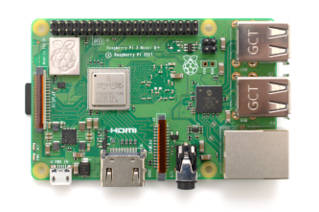
\includegraphics[width=\linewidth]{img/raspberry.png} &
					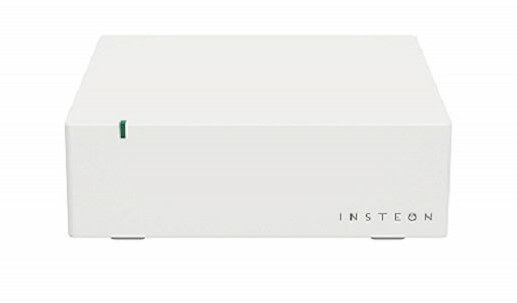
\includegraphics[width=\linewidth]{img/insteon_hw.png} & 
					\Includegraphics[width=\linewidth]{img/wink_hw.png} &
					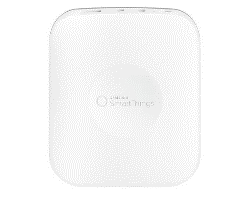
\includegraphics[width=\linewidth]{img/samsung_hw.png}
					\\\hline
					
					\textbf{Hub Price} & 25\$ & 80\$ & 99\$ & 70\$ \\\hline
					\textbf{Hardware Price} & parts are very cheap &  expensive parts & very expensive parts & expensive parts \\\hline
					\textbf{Flexibility} & any hardware that can be physically connected & 42 hardwares of basic variety\cite{insteon_p} & 102 hardwares of different variety\cite{wink_p} & only 6 hardwares support \cite{samsung_p} \\\hline
					
					\textbf{Installation \& Configuration Difficulty} & require one expert user. Easy control for all other users via mobile app & easy to install and control hardwares with mobile app  &easy to install and control hardwares with mobile app  & easy to install and control hardwares with mobile app
					\\\hline
				\end{tabularx}
			\end{center}
			\caption{Proposed \& Similar System Comparison}
			\label{table:compare}
		\end{table}
		\label{future}
		\paragraph{} Although similar systems already exists, our system has its own special advantages. The biggest being \textbf{hardware freedom}. In other systems, there exists a main hub receiving user command from the mobile app. So far, the ideas and implementation is identical. The previous systems require the consumer to by additional parts for it to work, such as special LED lights that needs installation or a small component controlling air conditioners. Those parts are usually limited in numbers, usage and can get very expensive fast. On the other hand, our system works with any hardware component as long as connecting it to the electrical circuit is possible.
		\paragraph{} However, this great flexibility comes with a great sacrifice: the steep learning curve. To keep the hardware prices as low as possible while maintaining high flexibility requires the buyer household to have one expert user. For example, in a family of four, all can control the AC. However, one of them must be an expert who can configure the hardware controlling the AC and adding it to raspberry pi manually. Of course, making it easier is possible, but it will result in a higher component cost and less flexibility as hardware components would need to be bought from our company (future implementation) in comparison to buying it from any cheap electronic store (current proposed solution).
		\paragraph{} \textit{figure \ref{fig:radar_diagram}} shows this relationship between flexibility, cost and usability for the three systems, our proposed solution and the merchant edition(future work).

		\begin{figure}[H]
			\centering
			\begin{subfigure}[b]{.4\linewidth}
				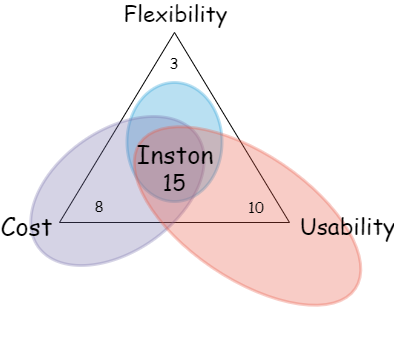
\includegraphics[width=\linewidth]{img/Inston.png}
				\caption{Insteon}
			\end{subfigure}
			\begin{subfigure}[b]{.4\linewidth}
				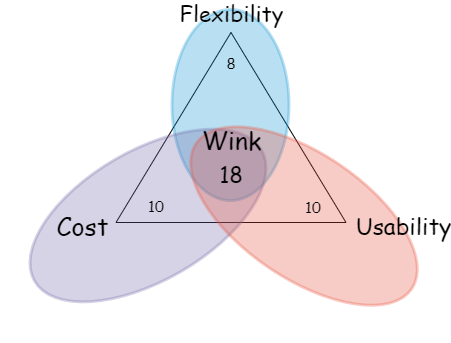
\includegraphics[width=\linewidth]{img/Wink.png}
				\caption{Wink}
			\end{subfigure}
			\begin{subfigure}[b]{.4\linewidth}
				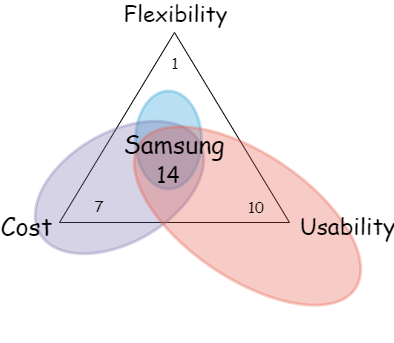
\includegraphics[width=\linewidth]{img/Samsung.png}
				\caption{Samsung}
			\end{subfigure}
			\begin{subfigure}[b]{.4\linewidth}
				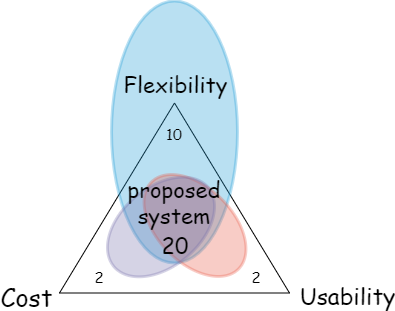
\includegraphics[width=\linewidth]{img/proposed.png}
				\caption{Proposed System}
			\end{subfigure}
			\begin{subfigure}[b]{.4\linewidth}
				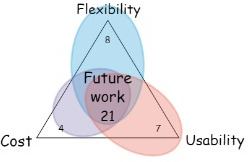
\includegraphics[width=\linewidth]{img/future.jpg}
				\caption{Future Work}
			\end{subfigure}
			
			\caption{Relationship between cost, flexibility and usability}
			\label{fig:radar_diagram}
		\end{figure}
		
		\newpage\section{System Design and Analysis}
		\paragraph{} Incremental model was used in this project. This model is a process of software development where requirements are broken down into multiple standalone modules of software development cycle. Incremental development is done in steps from analysis design, implementation, testing / verification, maintenance\cite{sdlc}. The reason this model was chosen is the pieces will be installed, tested and connected to the system gradually.
		
		\paragraph{} System requirements were gathered and selected  after discussing the proposed idea thoroughly. Top-down approach was used, in which we discussed the general goal of this project, then broke it down even further to smaller manageable units. \textit{Non-Functional Requirements} are shown in \textit{Table \ref{table:non-func}}. On the other hand, \textit{Functional Requirements} are realized through many diagrams. Each showing one side of the system. \textit{See Appendix \ref{appendix:diagram} for more diagrams.}
		

		% NON FUNCTIONAL
		\subsection{Non-Functional Requirements}
		\def\arraystretch{1.5}
		\begin{table}[H]
			\begin{center}
				\begin{tabularx}{\linewidth}{|c|X|}\hline
					\textbf{Requirement} & \textbf{Description}\\\hline
					\textbf{Availability} & The system shall not be shut down for maintenance for more than 1 minute. \\\hline
					\textbf{Usability} & Except the expert user, all other user of the system shall be able to use the system immediately without much training  \\\hline
					\textbf{Verifiability} & The system shall check the user identity. \\\hline
					\textbf{Performance and Delay} & The raspberry pi shall read user commands each 30 seconds to avoid delay or overhead in the system\\\hline
					\textbf{Flexibility} & Any hardware component, such as linear solenoid or an infra-red controller, can be added to the system as long as it can be connected to the electric circuit.  \\\hline
					\textbf{Security} & Each user can only communicate with assigned raspberry pi. In a similar manner, raspberry pi only reads commands meant for it and not for other ones.  \\\hline
					\textbf{Efficiency} & The web server cleans the database and deletes any unneeded rows routinely.  \\\hline
				\end{tabularx}
			\end{center}
			\caption{Non-functional requirements}
			\label{table:non-func}
		\end{table}
		\paragraph{} \textit{Table \ref{table:non-func}} shows the non-functional requirements for the system and their description. The most important requirement is flexibility, as it is the core feature differentiating the proposed system from other systems. Next comes security and verifiability. They guarantee that no intruders are going to interrupt the system even if they communicated with the REST API directly without the android app because they won't be authorized -or authenticated- to enter the system. The other requirements are manly for performance and ease of use. 
		
	\subsection{System Architecture}
	\paragraph{} The proposed project has 4 tiers. The Android App, the web app and finally the raspberry pi script and finally the system database. The android app works as the user interface. The raspberry pi app is the one responsible for controlling the actual hardwares. The web app  works as a medium for managing user requests and raspberry pi's response. Finally, the database that stores these data.
.
	\paragraph{} \textit{Figure \ref{fig:diagram_architecture}} shows the four-tier architecture explained above. In our system, the best architecture to use is four-tier architecture because of it is flexibility and scalability to add multiple services. Also, it adopts users’ experiences that are fast, responsive, and tailored unique needs. Furthermore, multi-tier architecture also reduces traffic on the network\cite{architecture}.
	\begin{figure}[H]
		\centering
		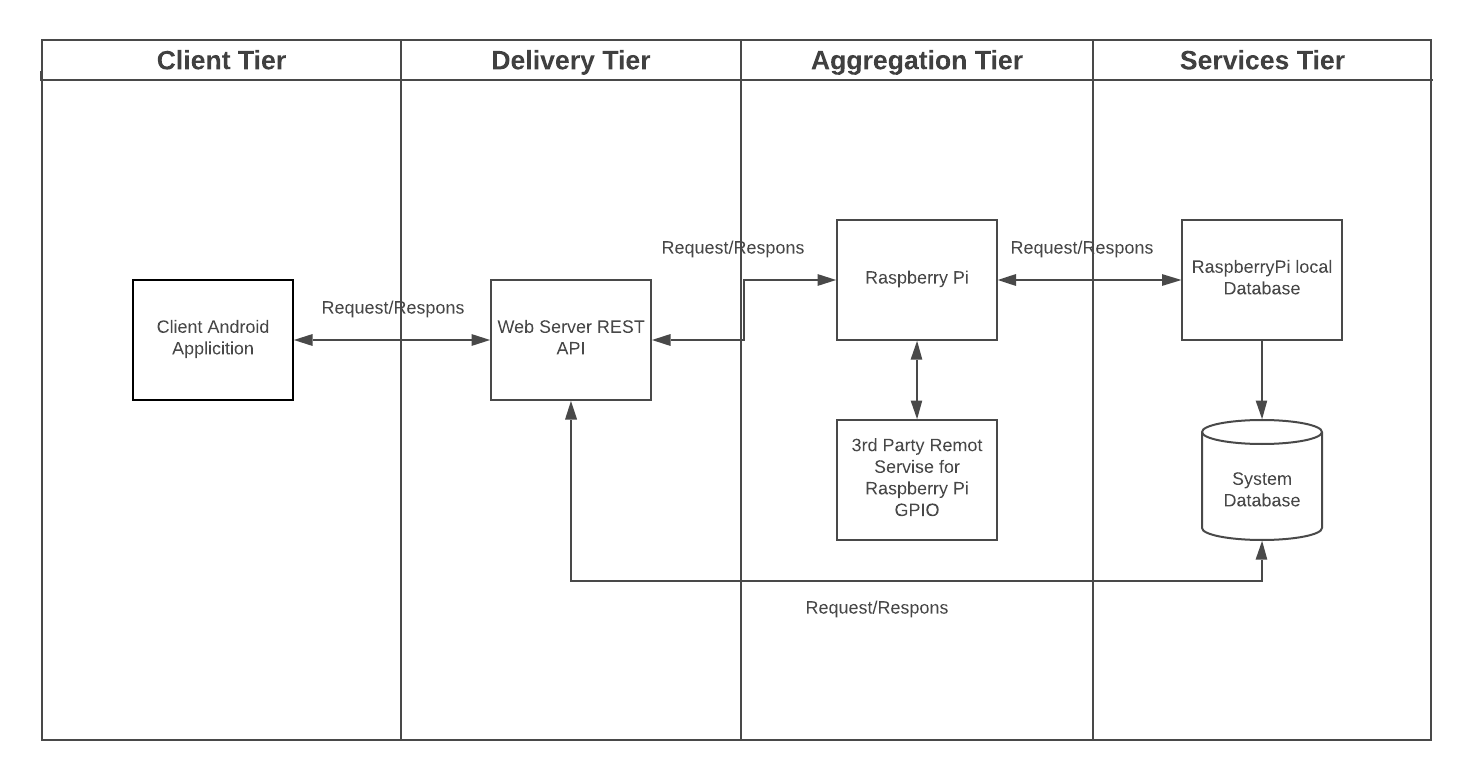
\includegraphics[width=\linewidth]{img/diagram_architecture.png}
		\caption{Architecture Diagram}
		\label{fig:diagram_architecture}
	\end{figure}

	
	% ERD
	\newpage\subsection{Entity Relationship Diagram}
	
	\textit{Figure \ref{fig:erd} shows the Entity-relationship diagram.} 
	\begin{figure}[H]
		\begin{subfigure}[b]{\linewidth}
			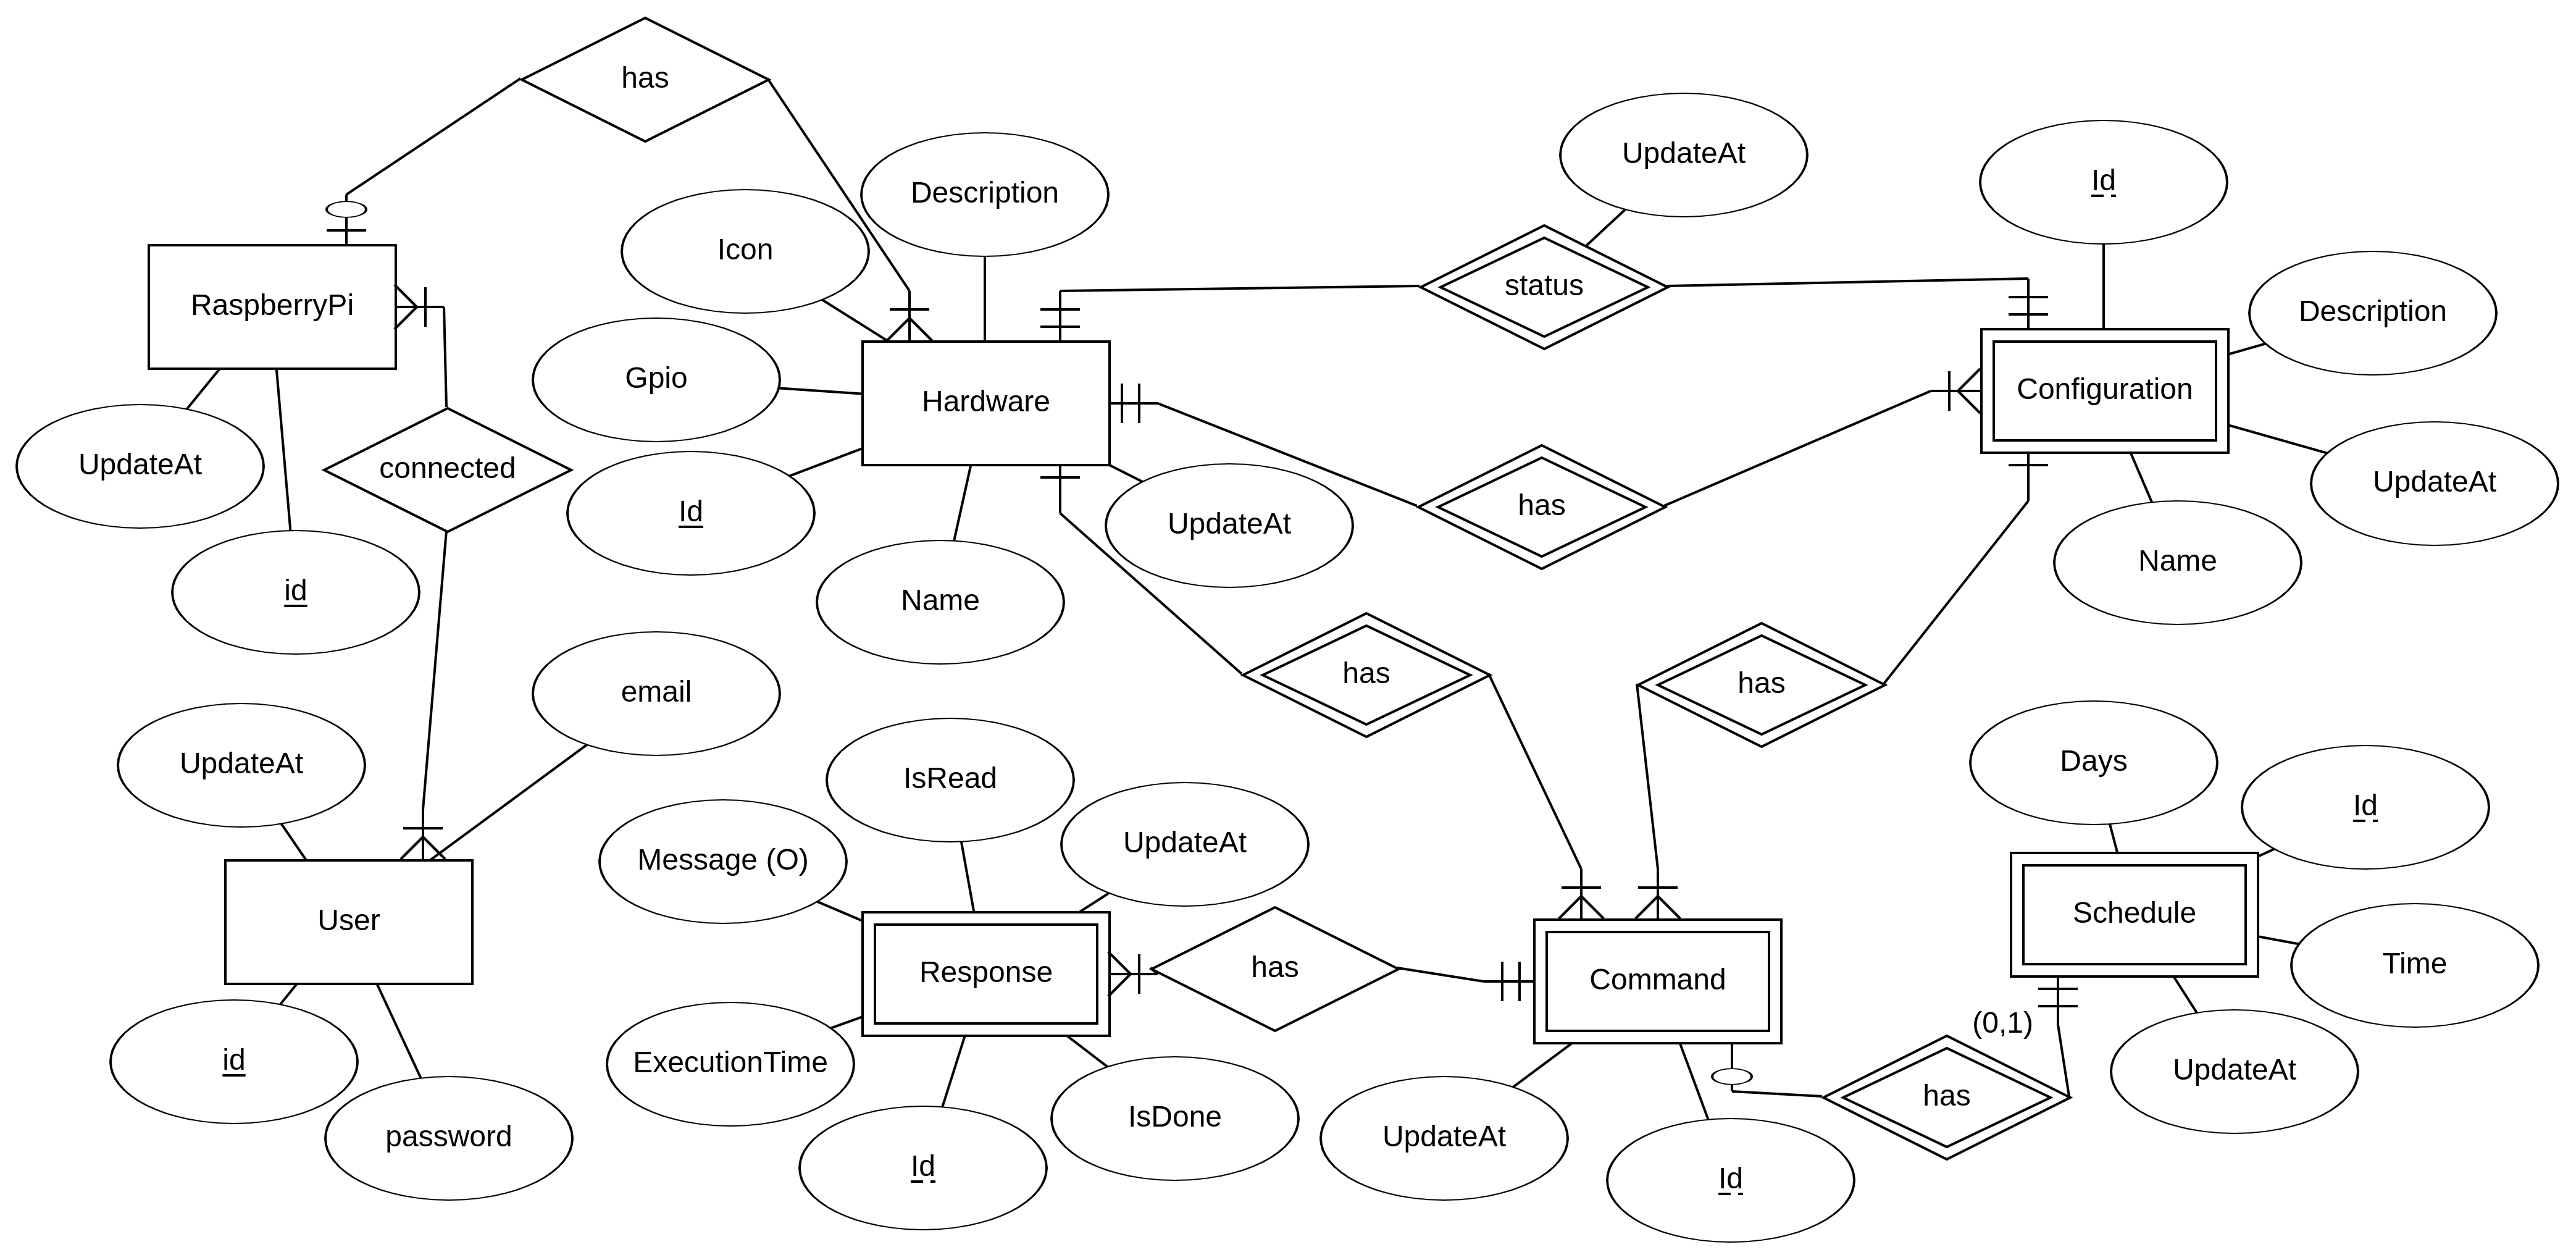
\includegraphics[width=\linewidth]{img/diagram_er1.png}
			\caption{System database}
		\end{subfigure}
		
		\begin{subfigure}[b]{\linewidth}
			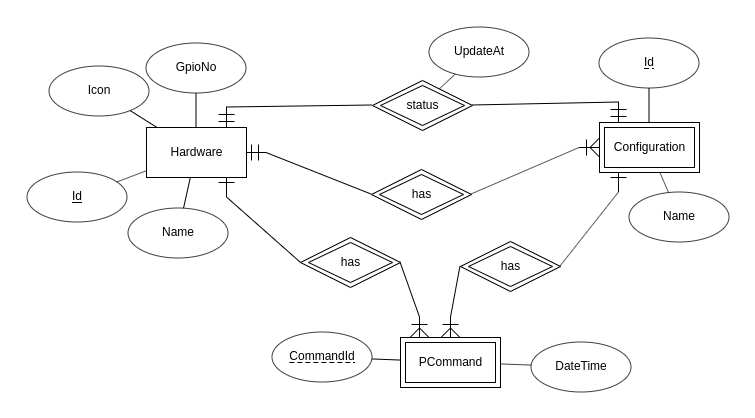
\includegraphics[width=\linewidth]{img/diagram_er2.png}
			\caption{Local queue}
		\end{subfigure}
		\caption{Entity-relationship diagrams}
		\label{fig:erd}
	\end{figure}
	
	


		\newpage\section{Results and Future Works}
		\paragraph{} The following are the main input and output screens
		\subsection{Login Screen}
		\paragraph{} First, the user is required to login or register before using the system. \textit{Figure \ref{output:login}} shows the login interface.
		\begin{figure}[H]
			\centering
			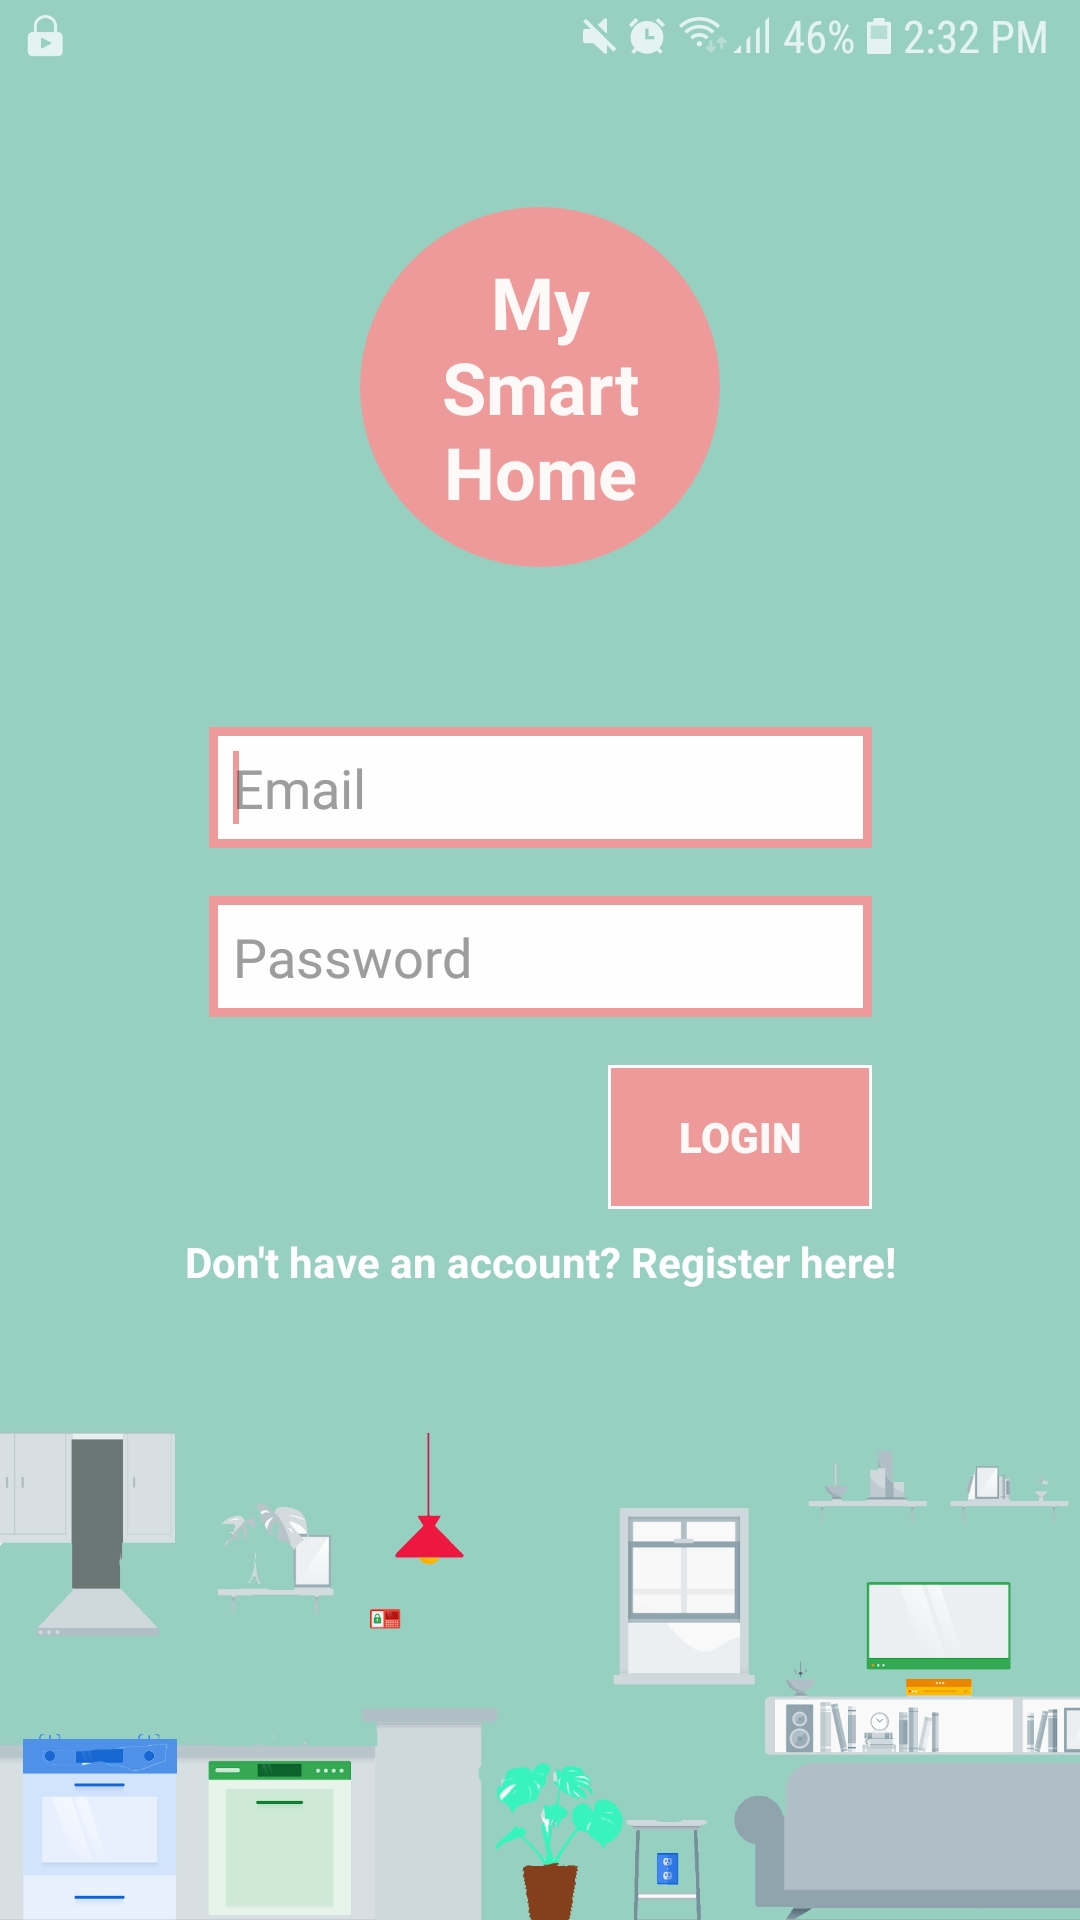
\includegraphics[width=.5\linewidth]{img/output_login.jpg}
			\caption{I/O: Login Screen}
			\label{output:login}
		\end{figure}
		
		\newpage\subsection{Raspberry Pi Screen}
		\paragraph{} After successful login, the user is redirected to the raspberry pi's list of connected devices. \textit{Figure \ref{output:rp}} shows the Raspberry Pi interfaces. 
		\begin{figure}[H]
			\centering
			\begin{subfigure}[b]{.4\linewidth}
				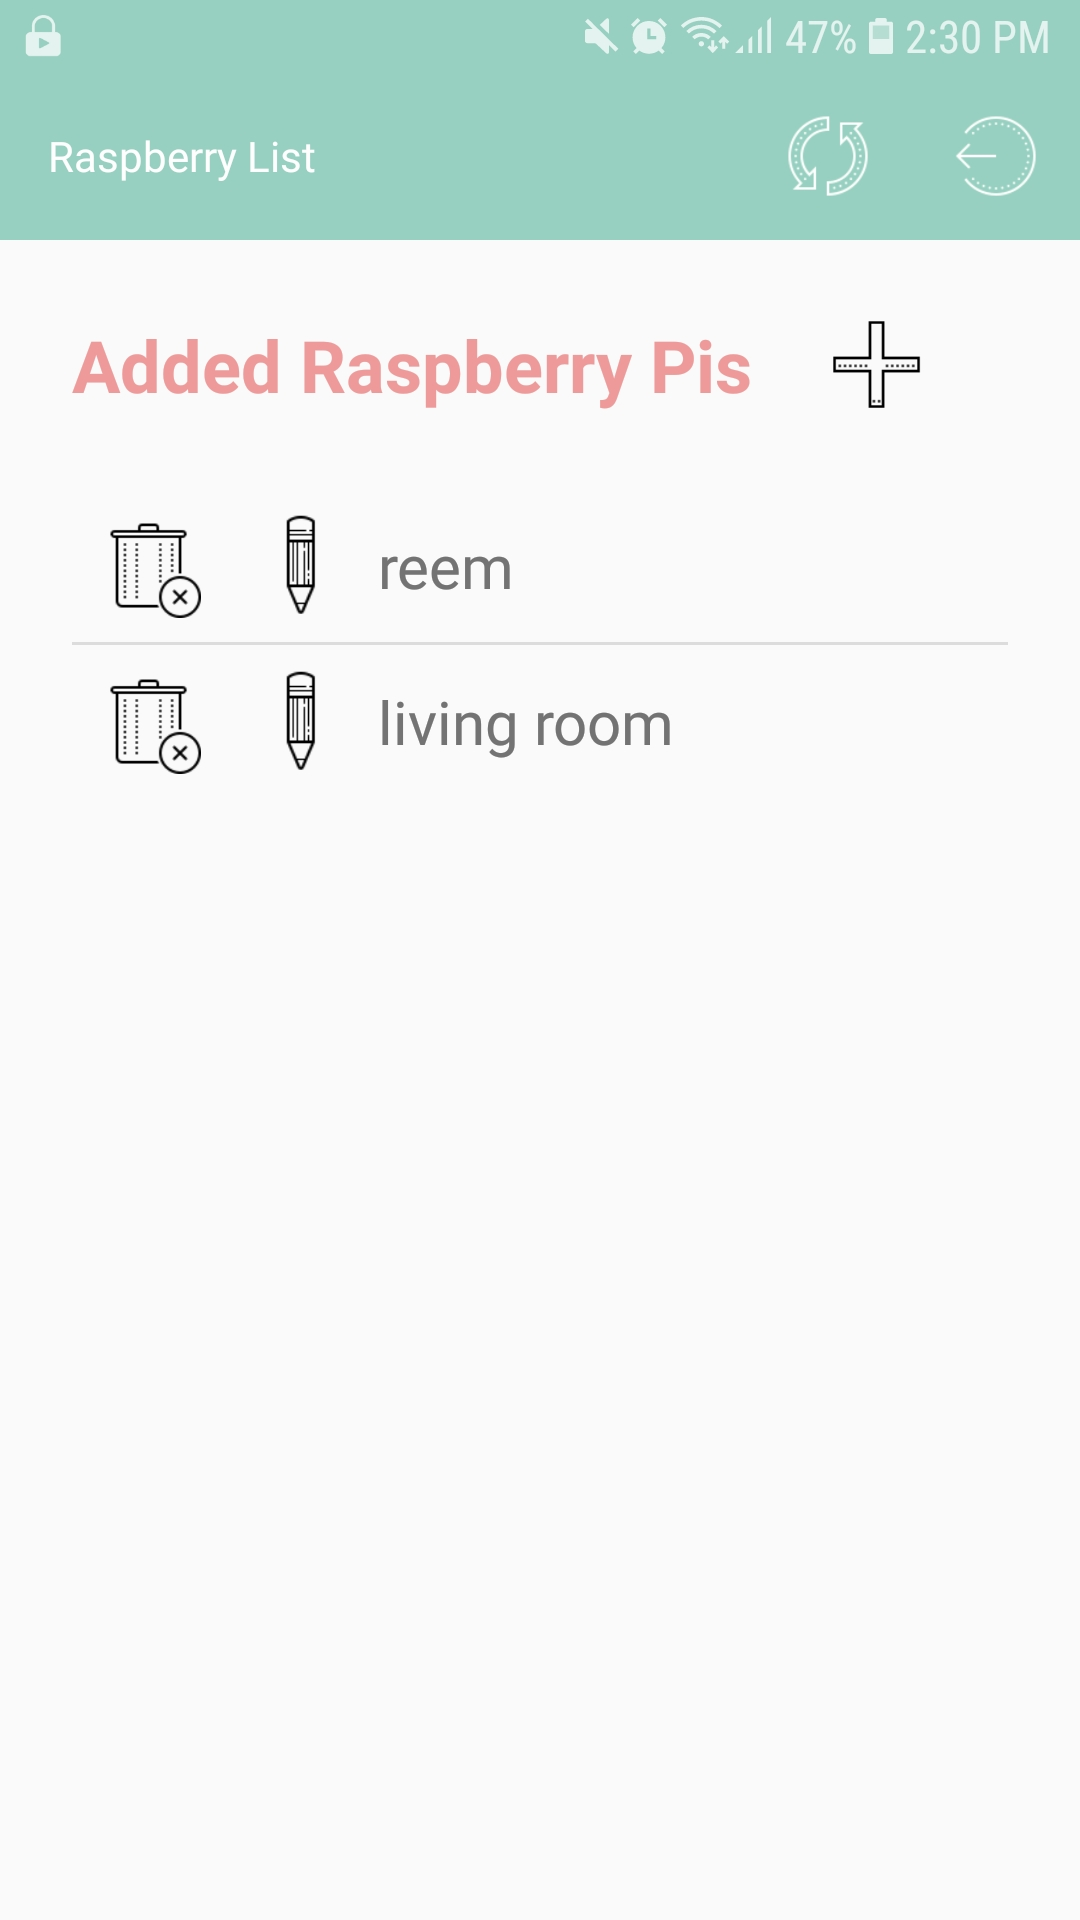
\includegraphics[width=\linewidth]{img/output_raspberry_list.jpg}
				\caption{I/O: Raspberry Pi List}
			\end{subfigure}
			\begin{subfigure}[b]{.4\linewidth}
				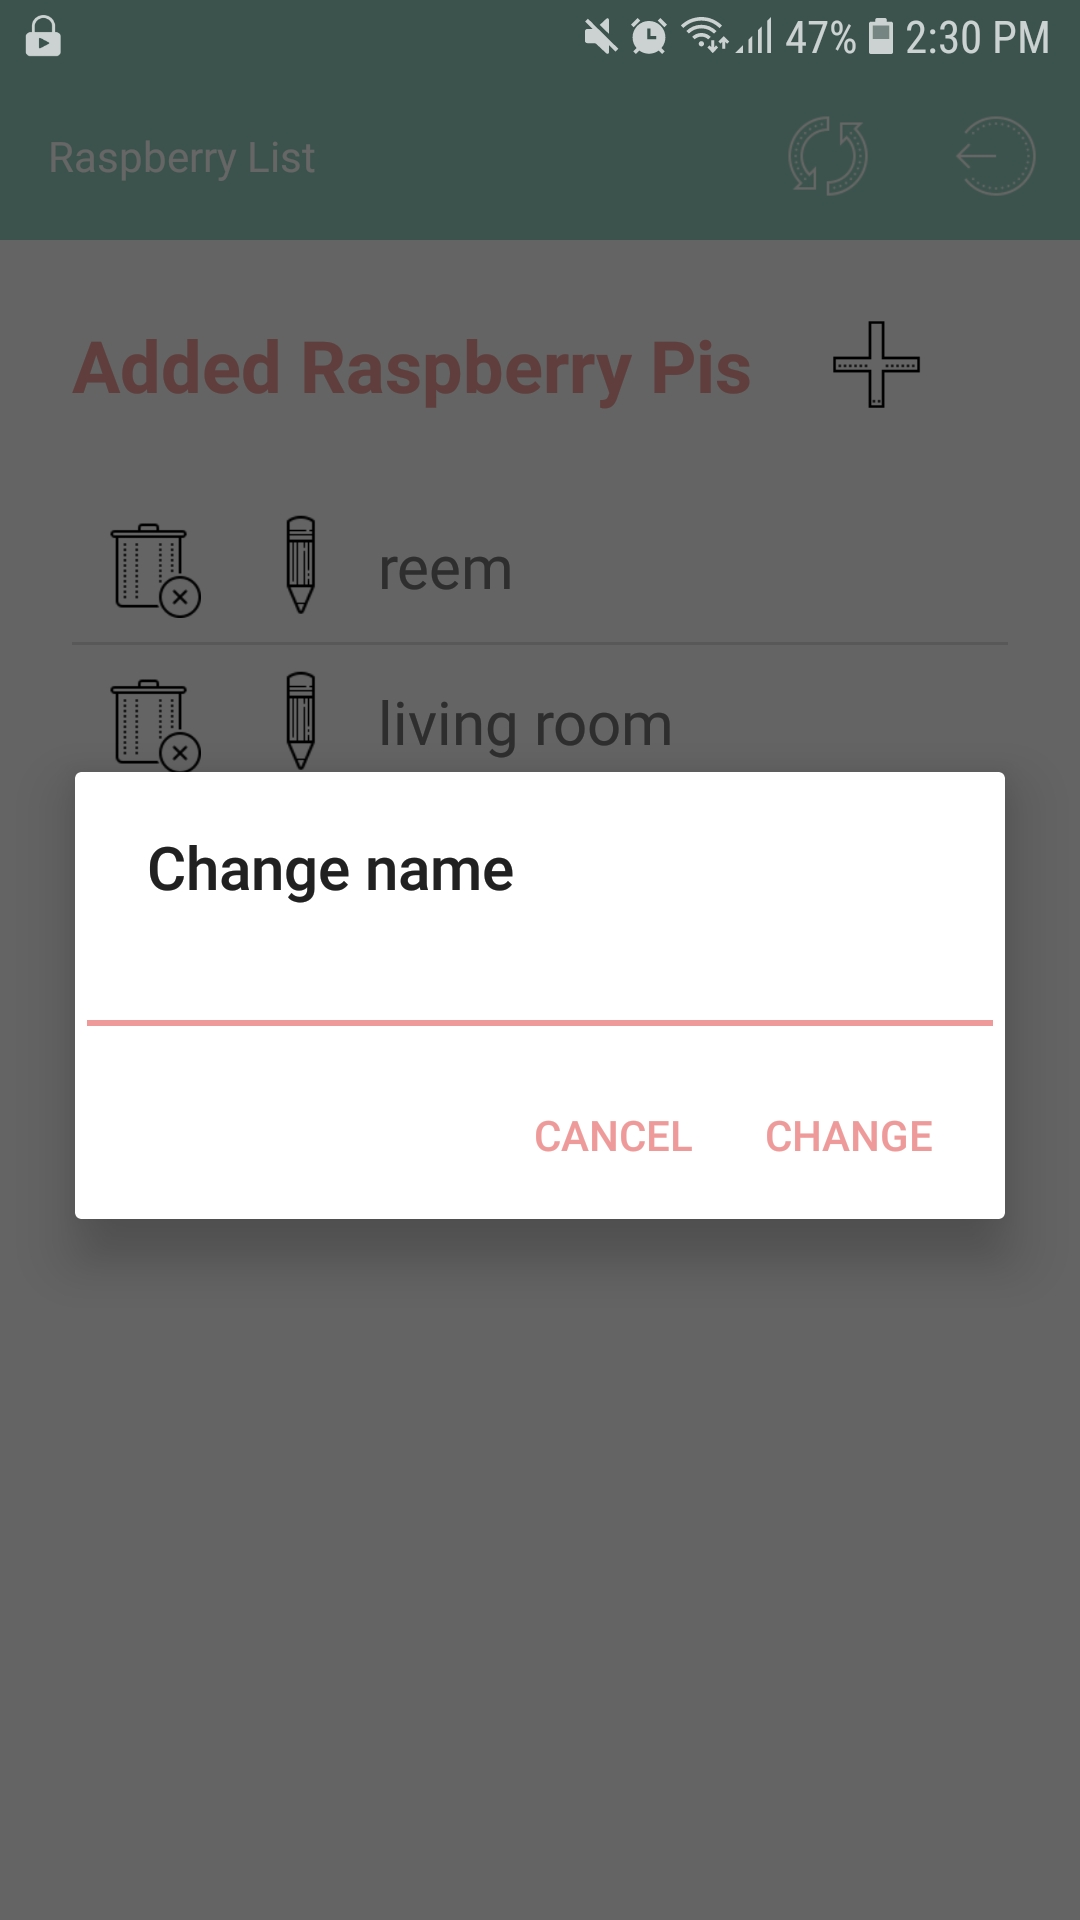
\includegraphics[width=\linewidth]{img/output_raspberry_edit.jpg}
				\caption{I/O: Raspberry Pi Edit}
			\end{subfigure}
			\caption{I/O: Raspberry Pi Screens}
			\label{output:rp}
		\end{figure}
		
		\newpage\subsection{Hardware Screen}
		\paragraph{} After clicking on one of the raspberry pi's, the hardware list appears. \textit{Figure \ref{output:hardware}} shows the Hardware interfaces. 
		\begin{figure}[H]
			\centering
			\begin{subfigure}[b]{.35\linewidth}
				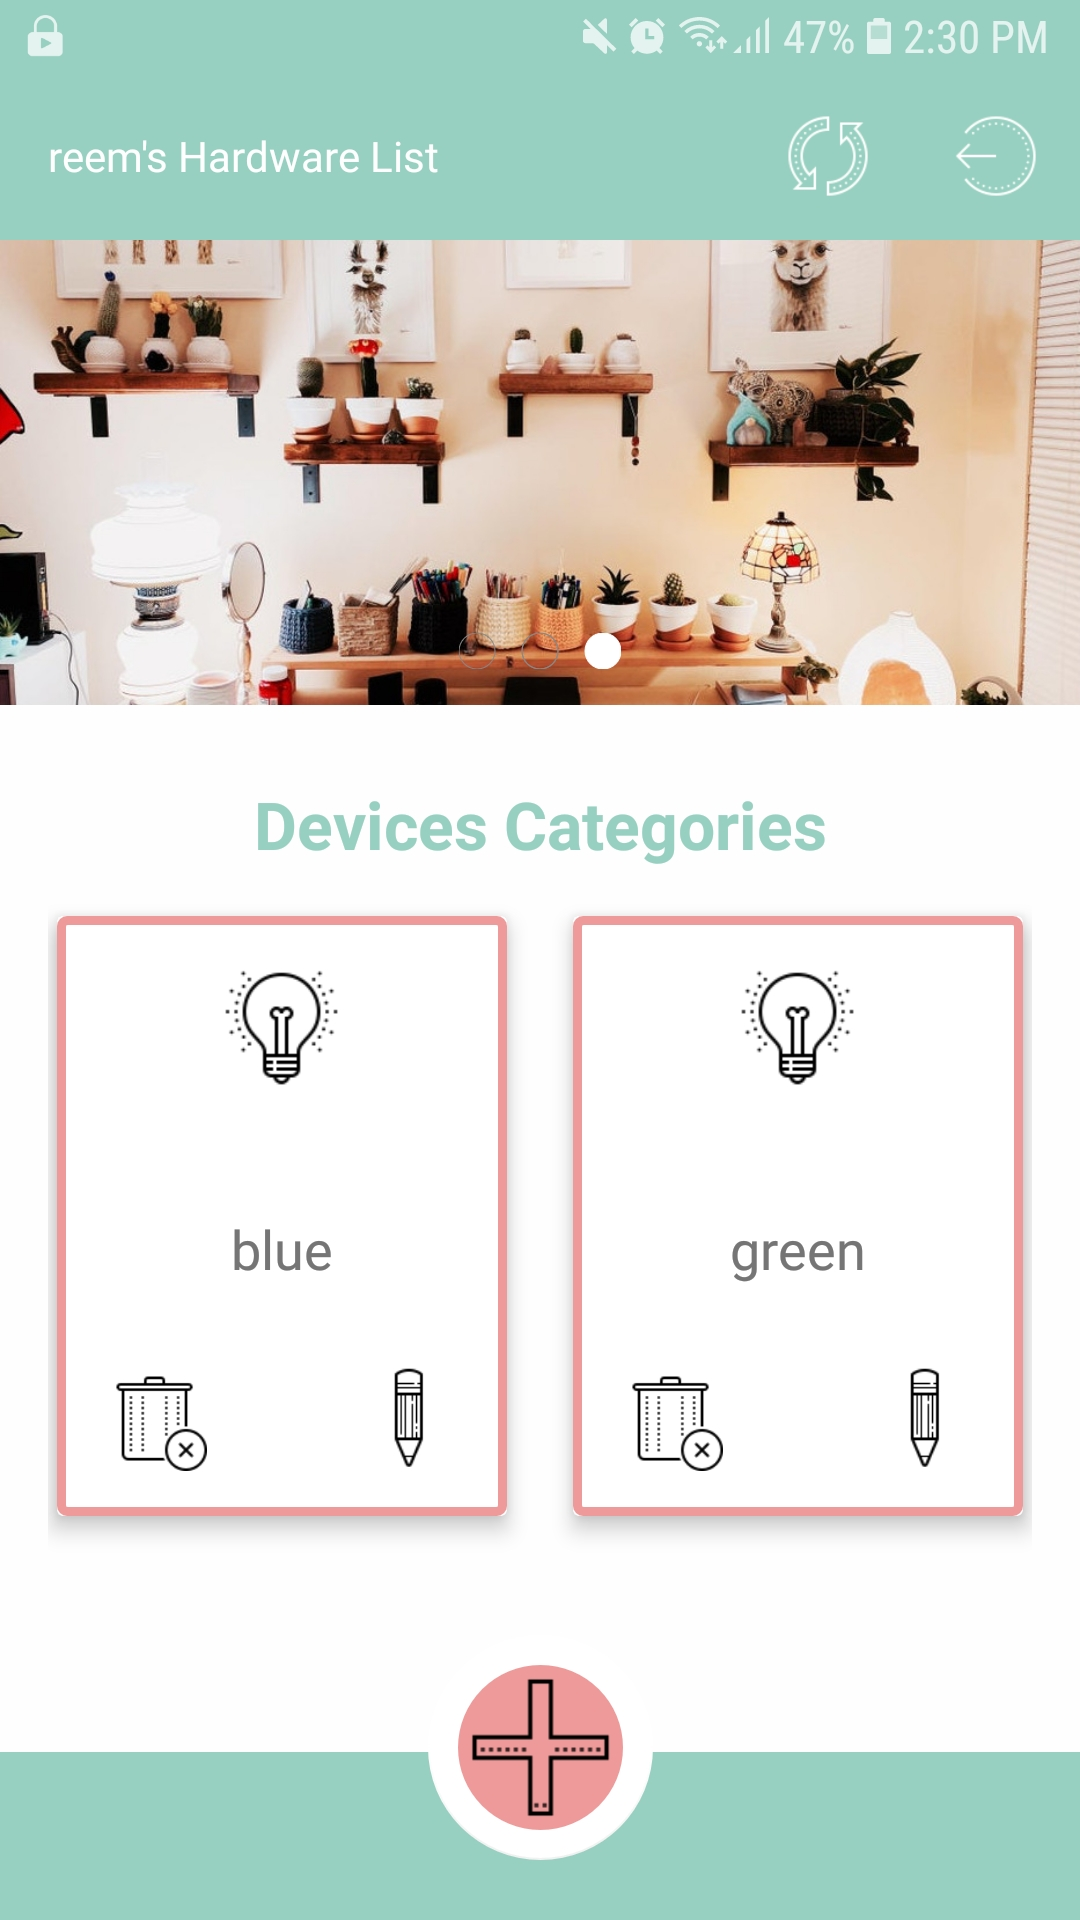
\includegraphics[width=\linewidth]{img/output_hardware_list.jpg}
				\caption{I/O: Hardware List}
			\end{subfigure}
			\begin{subfigure}[b]{.35\linewidth}
				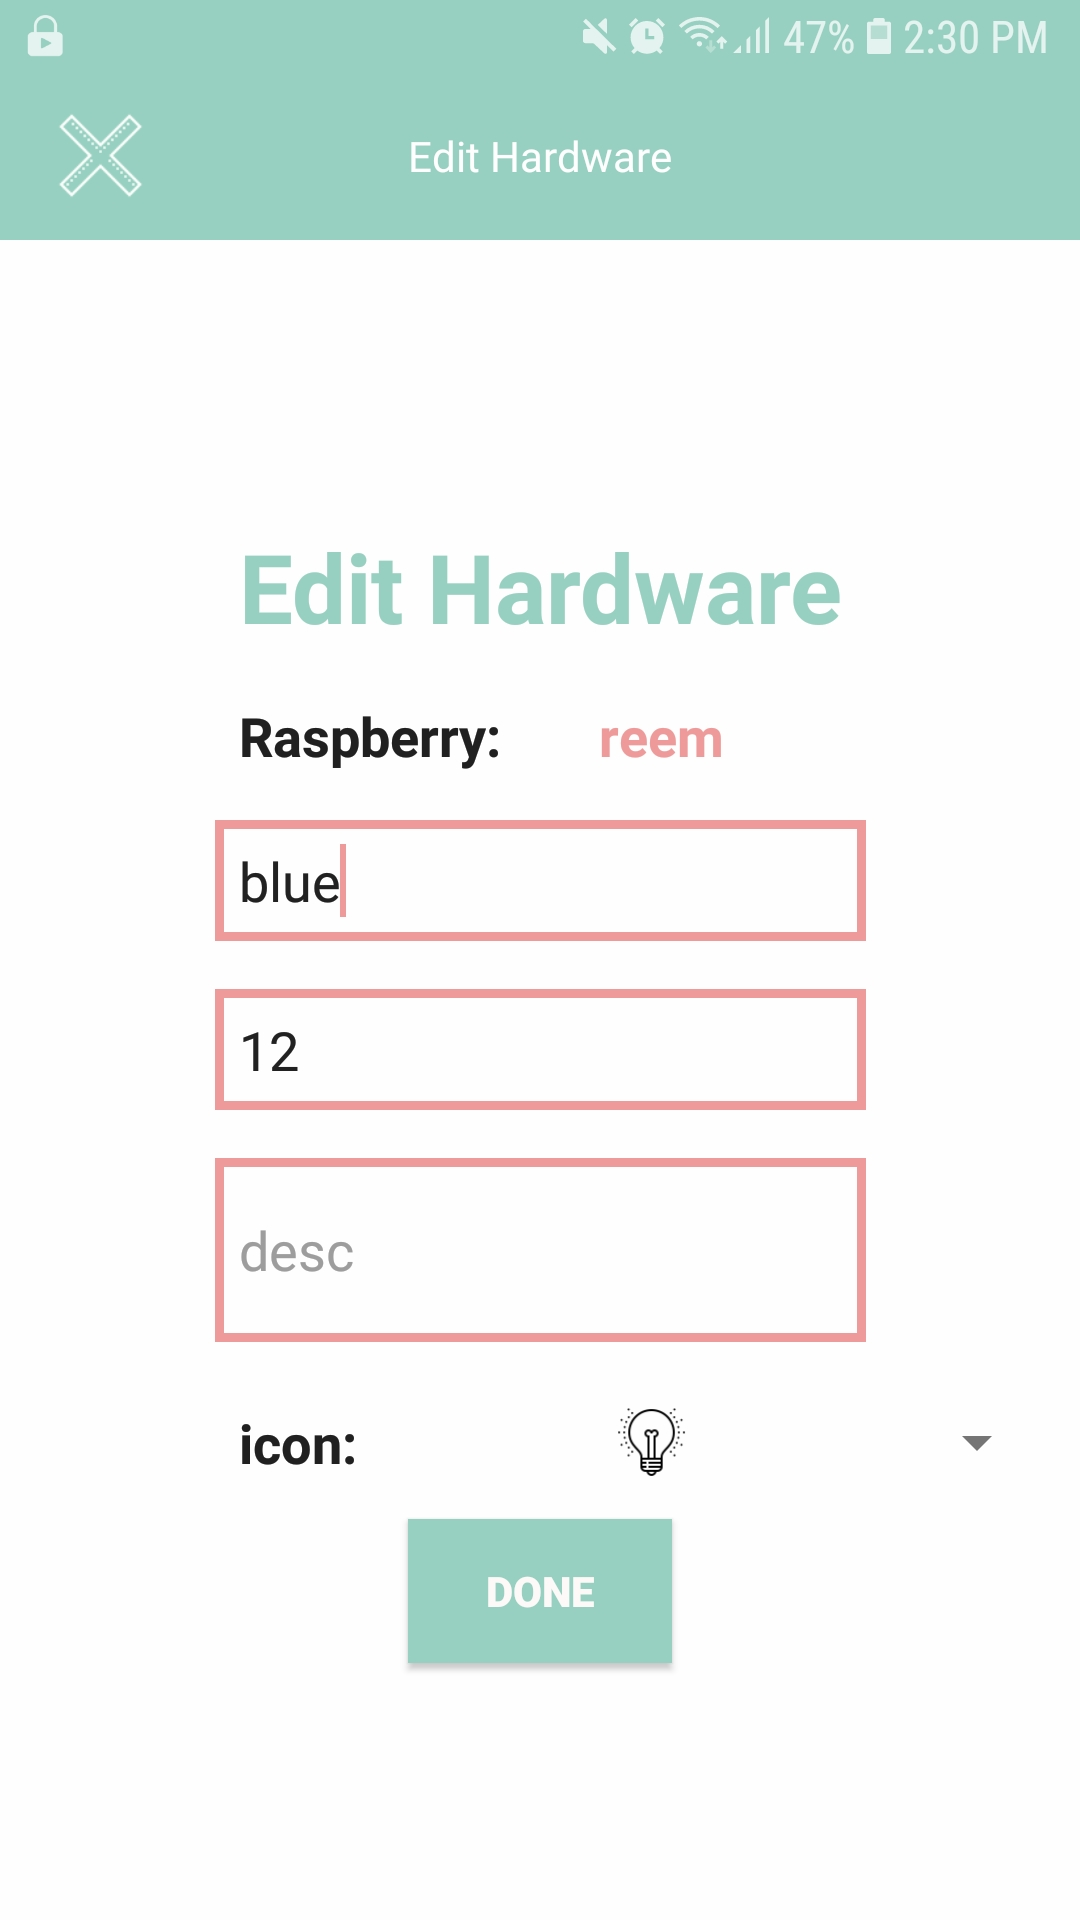
\includegraphics[width=\linewidth]{img/output_hardware_edit.jpg}
				\caption{I/O: Hardware Edit}
			\end{subfigure}
			\begin{subfigure}[b]{.35\linewidth}
				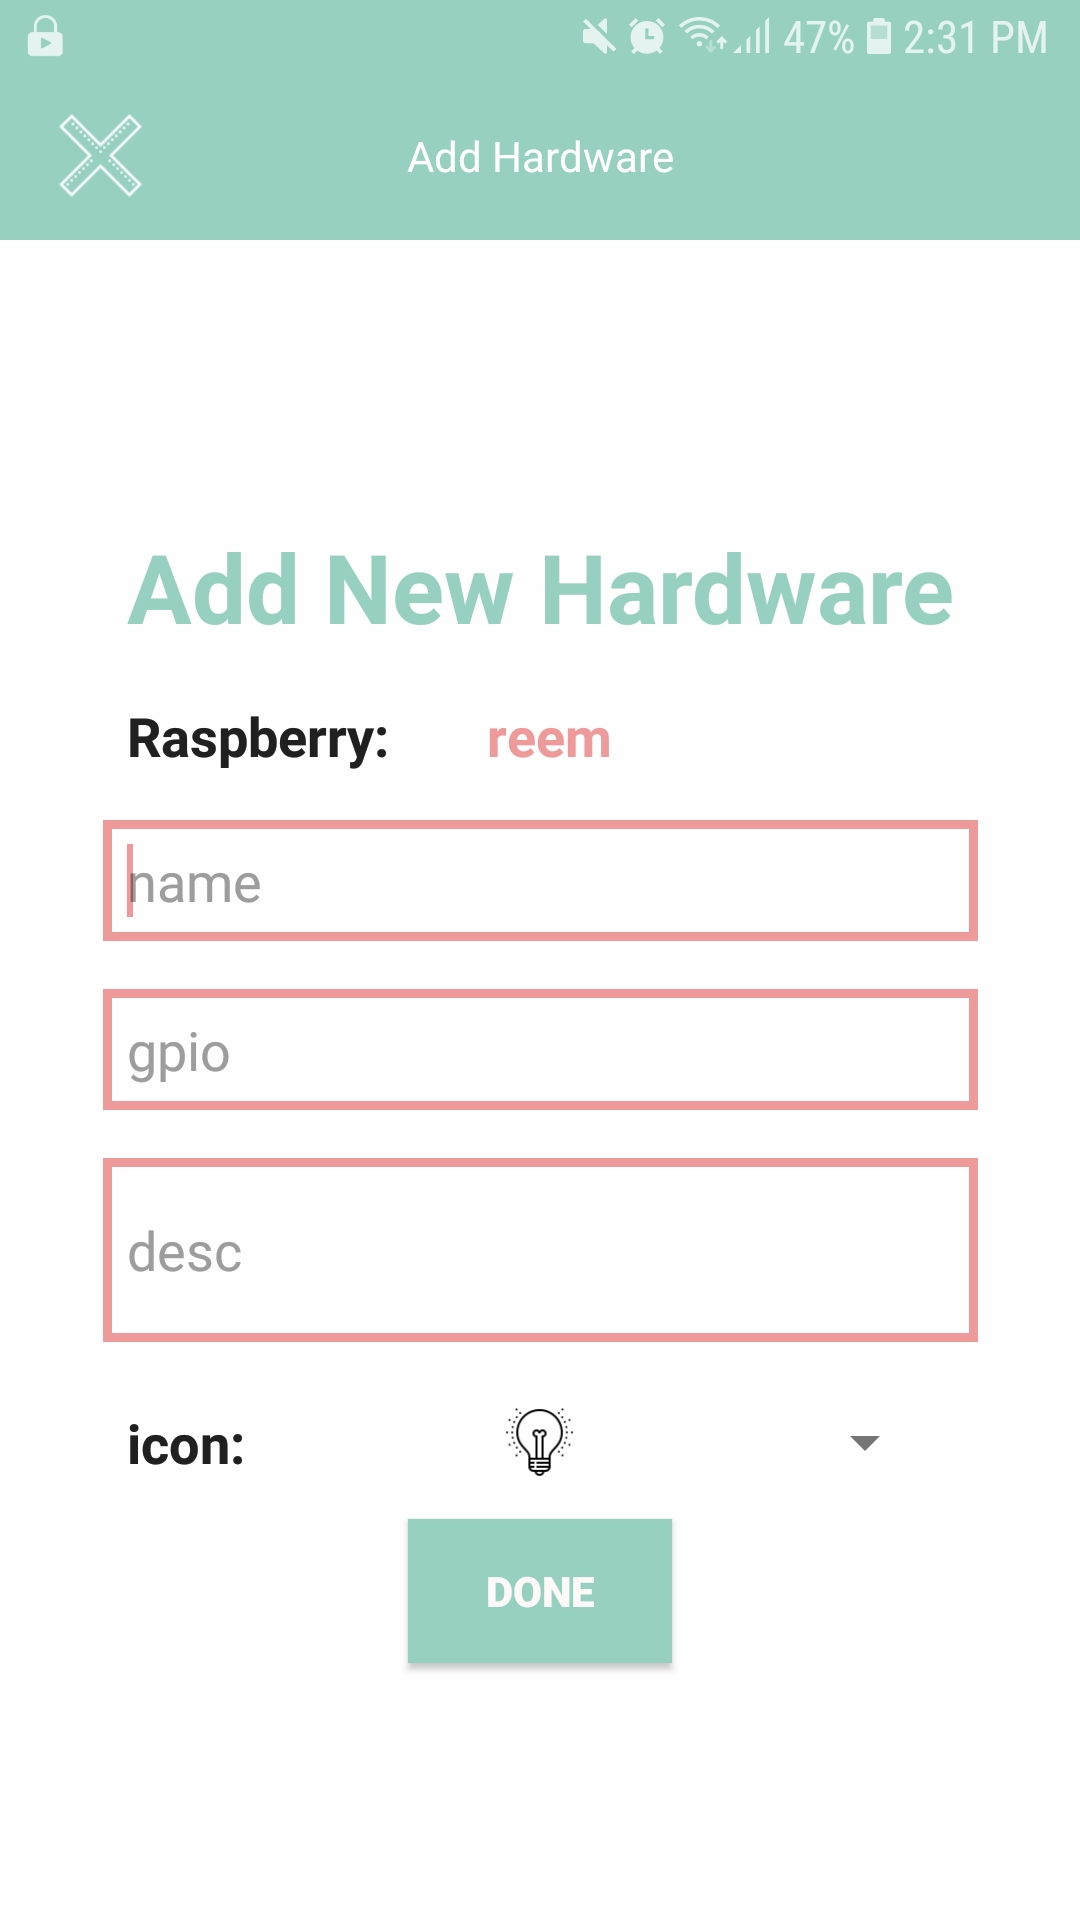
\includegraphics[width=\linewidth]{img/output_hardware_new.jpg}
				\caption{I/O: Hardware Create}
			\end{subfigure}
			\caption{I/O: Hardware Screens}
			\label{output:hardware}
		\end{figure}
		
		\newpage\subsection{Command \& Schedule Screen}
		\paragraph{} For each hardware, a user can create a command and see the command list. \textit{Figure \ref{output:command}} shows the Command and Schedule interfaces. 
		\begin{figure}[H]
			\centering
			\begin{subfigure}[b]{.35\linewidth}
				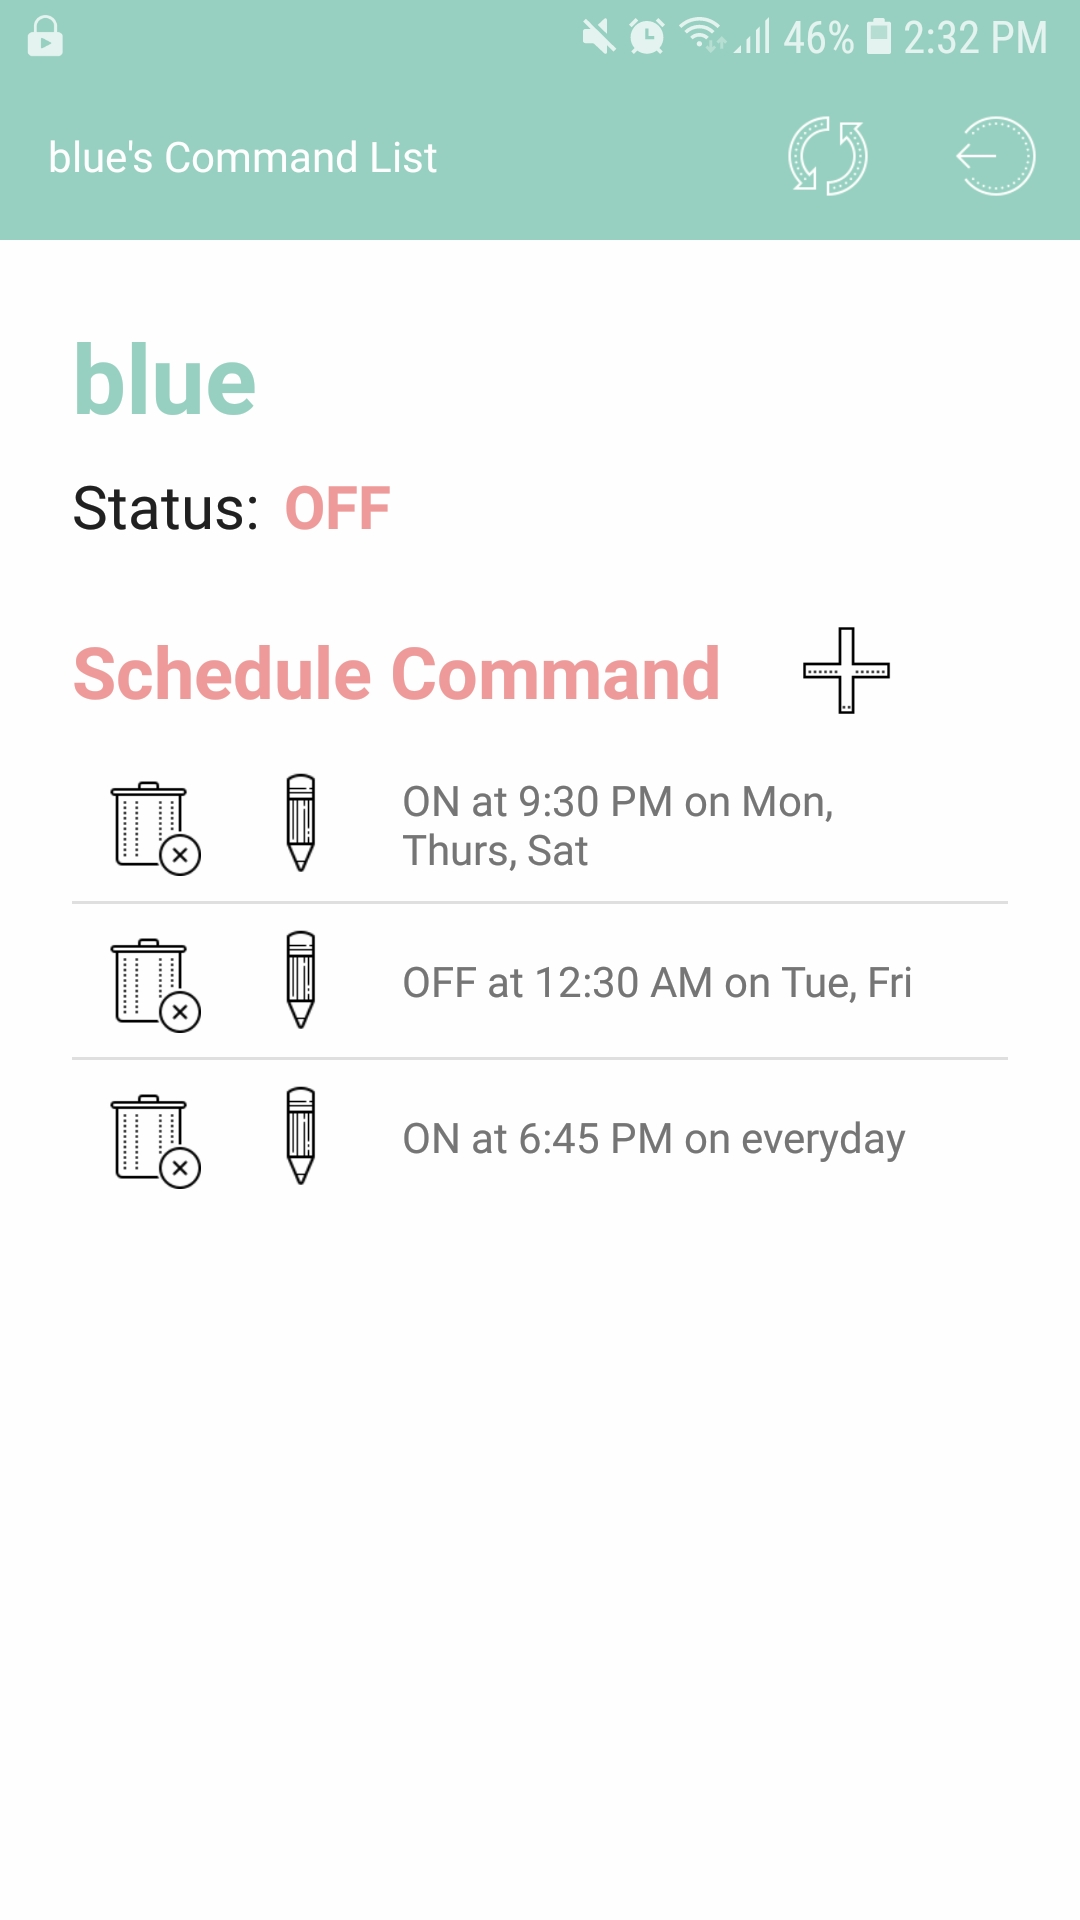
\includegraphics[width=\linewidth]{img/output_command_list.jpg}
				\caption{I/O: Command List}
			\end{subfigure}
			\begin{subfigure}[b]{.35\linewidth}
				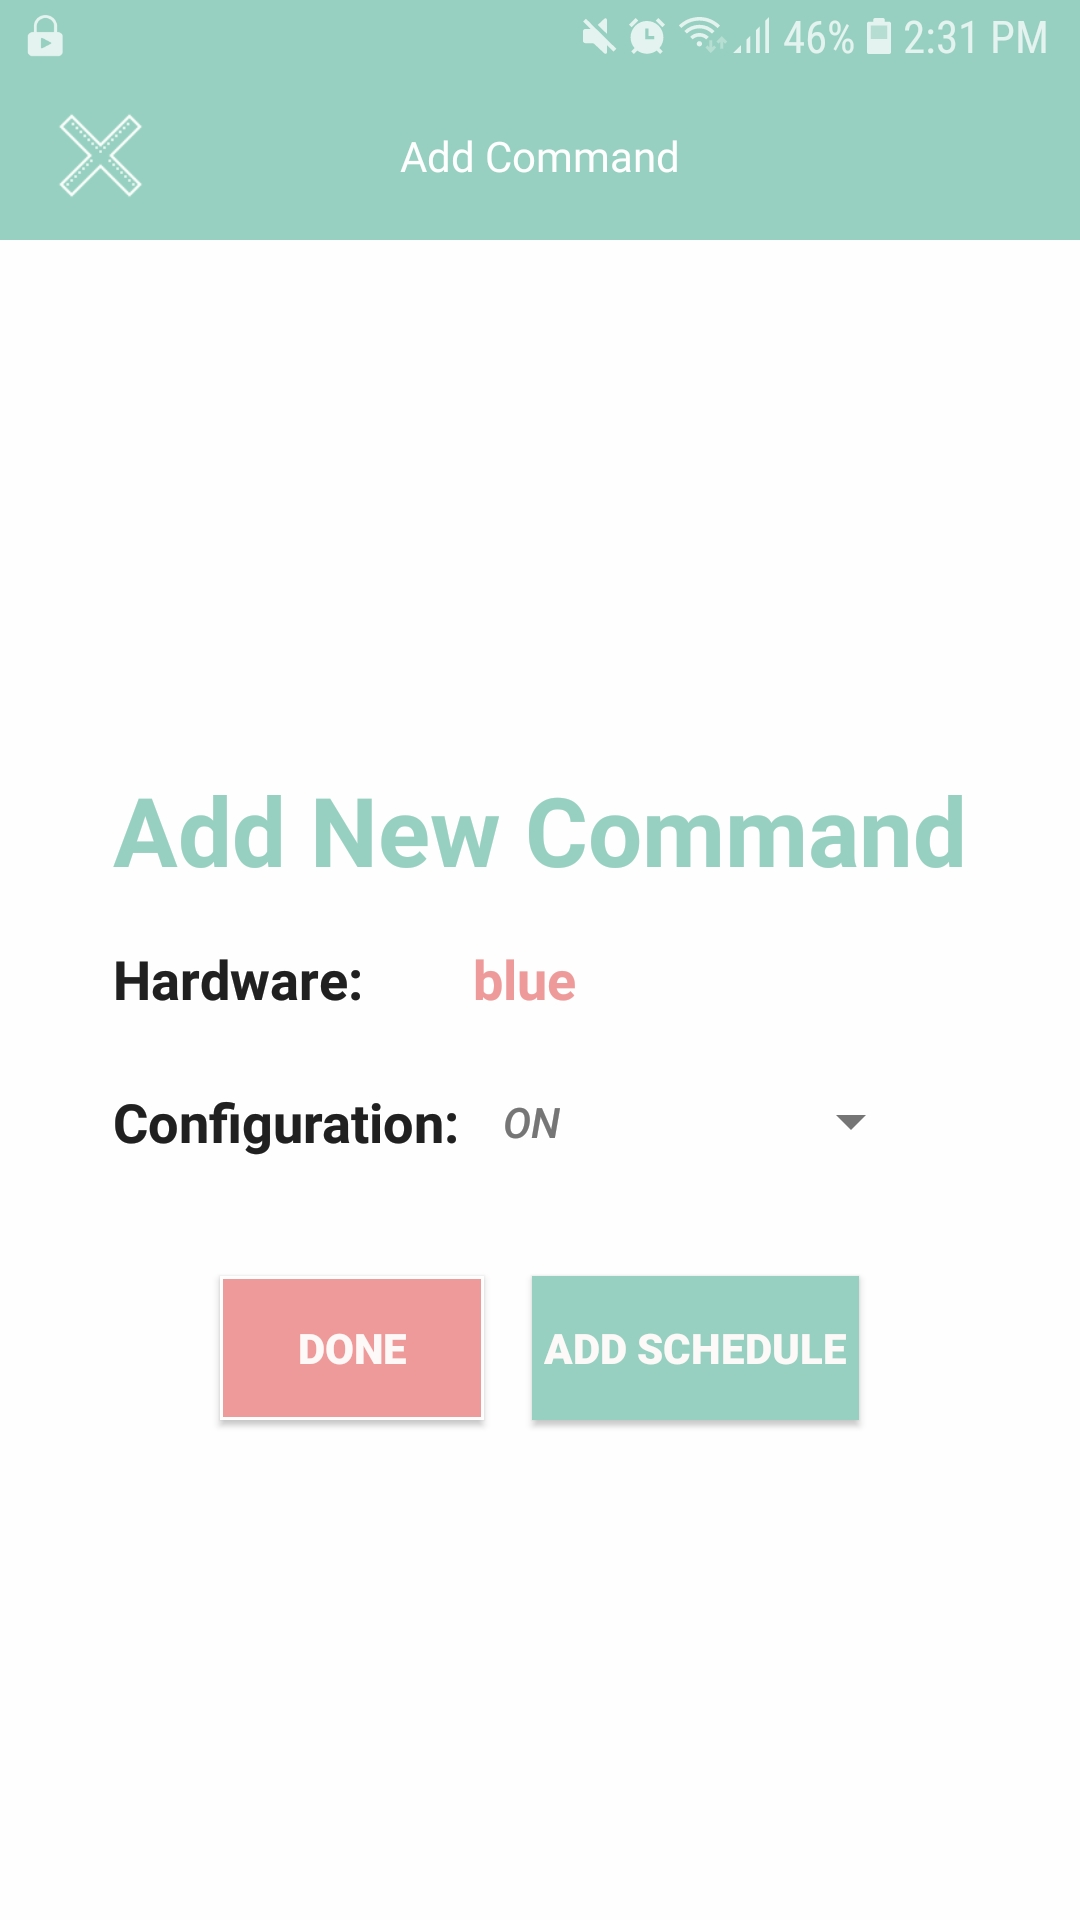
\includegraphics[width=\linewidth]{img/output_command_new.jpg}
				\caption{I/O: Command Create}
			\end{subfigure}
			\begin{subfigure}[b]{.35\linewidth}
				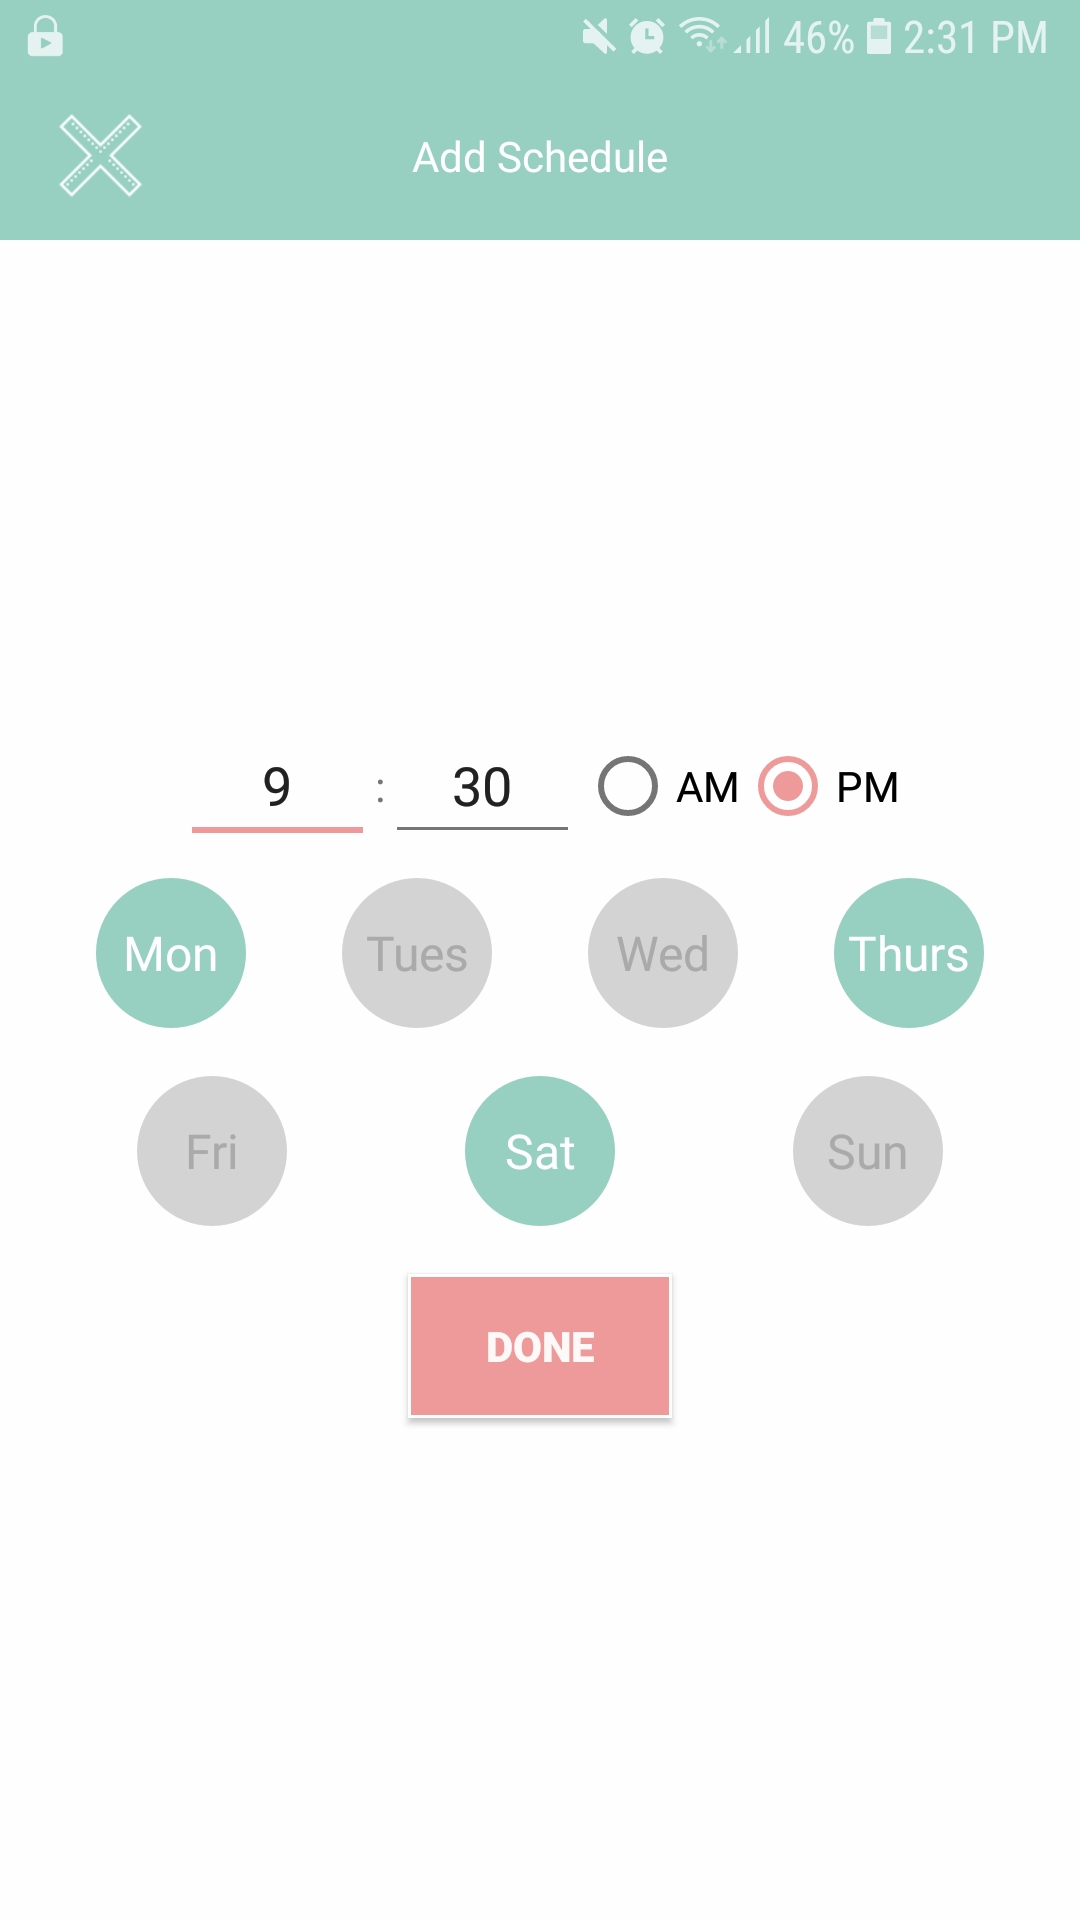
\includegraphics[width=\linewidth]{img/output_schedule.jpg}
				\caption{I/O: Schedule Create}
			\end{subfigure}
			\caption{I/O: Command Screens}
			\label{output:command}
		\end{figure}
		
		\subsection{Future Work}
		\paragraph{} As with every system, there are definitely improvements and enhancements to be made. Besides what was mentioned in \textit{Section \ref{future}}, more configuration can be added to hardwares, like multiple LED colors or different fan speeds. Also, making it wireless will further reduce its cost and remove the hassle of wires connecting, maintenance and wires going bad. 
		
		\section{Conclusion}
		\paragraph{}In summary, this project aimed to create a system that controls electronic household items from afar. In short, an android application was used as an interface for the user to issue control commands, which are in turn sent to and stored in the server. They are gotten from the server by a small computer (Raspberry Pi) that controls an electric circuit, to which the desired household items are connected and manipulated as per the commands. The project is a direct application of the concept of Internet of things and automated house systems.
		
		
		
		\bibliographystyle{ieeetr}
		\bibliography{References}
		
		
		\clearpage
		\section*{Appendices}
		\appendix

		\section{Similar systems hub design}
		\label{appendix:similar_system_comparision}
		\begin{figure}[H]
			\begin{subfigure}[b]{.5\linewidth}
				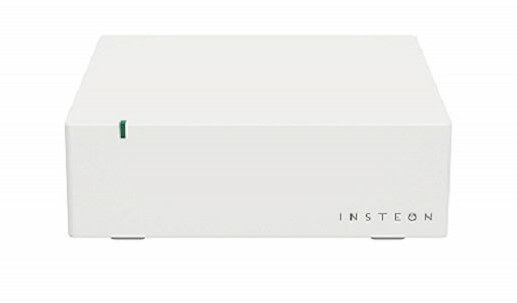
\includegraphics[width=\linewidth]{img/insteon_hw.png}
				\caption{Insteon}
			\end{subfigure}
			\begin{subfigure}[b]{.5\linewidth}
				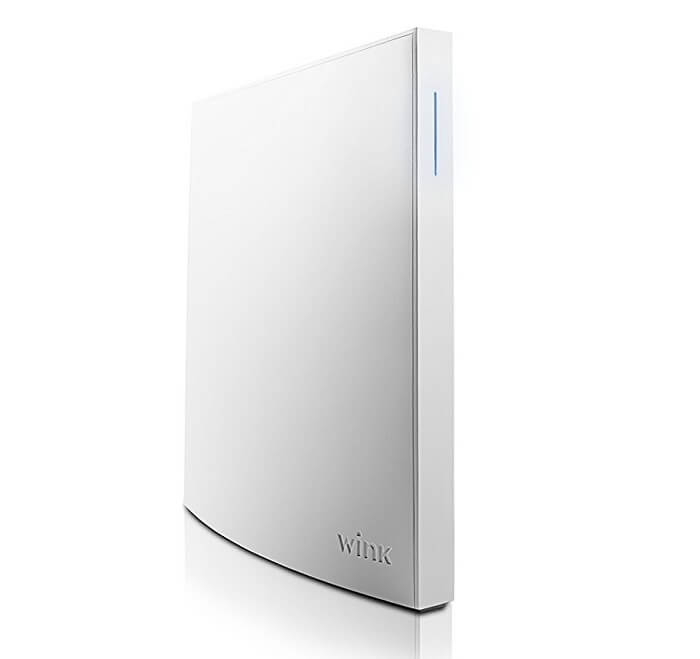
\includegraphics[width=\linewidth]{img/wink_hw.png}
				\caption{Wink}
			\end{subfigure}
			\begin{subfigure}[b]{.5\linewidth}
				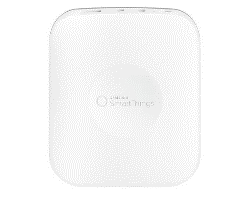
\includegraphics[width=\linewidth]{img/samsung_hw.png}
				\caption{Samsung}
			\end{subfigure}
			\begin{subfigure}[b]{.5\linewidth}
				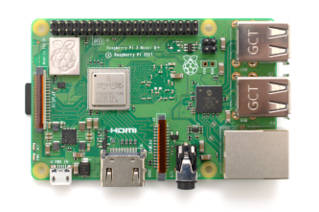
\includegraphics[width=\linewidth]{img/raspberry.png}
				\caption{Raspberry Pi}
			\end{subfigure}
			\caption{Similar systems: hub design}
		\end{figure}

		\section{Diagrams}
		\label{appendix:diagram}
		\subsection{Use-Case Diagram}
			\begin{figure}[H]
			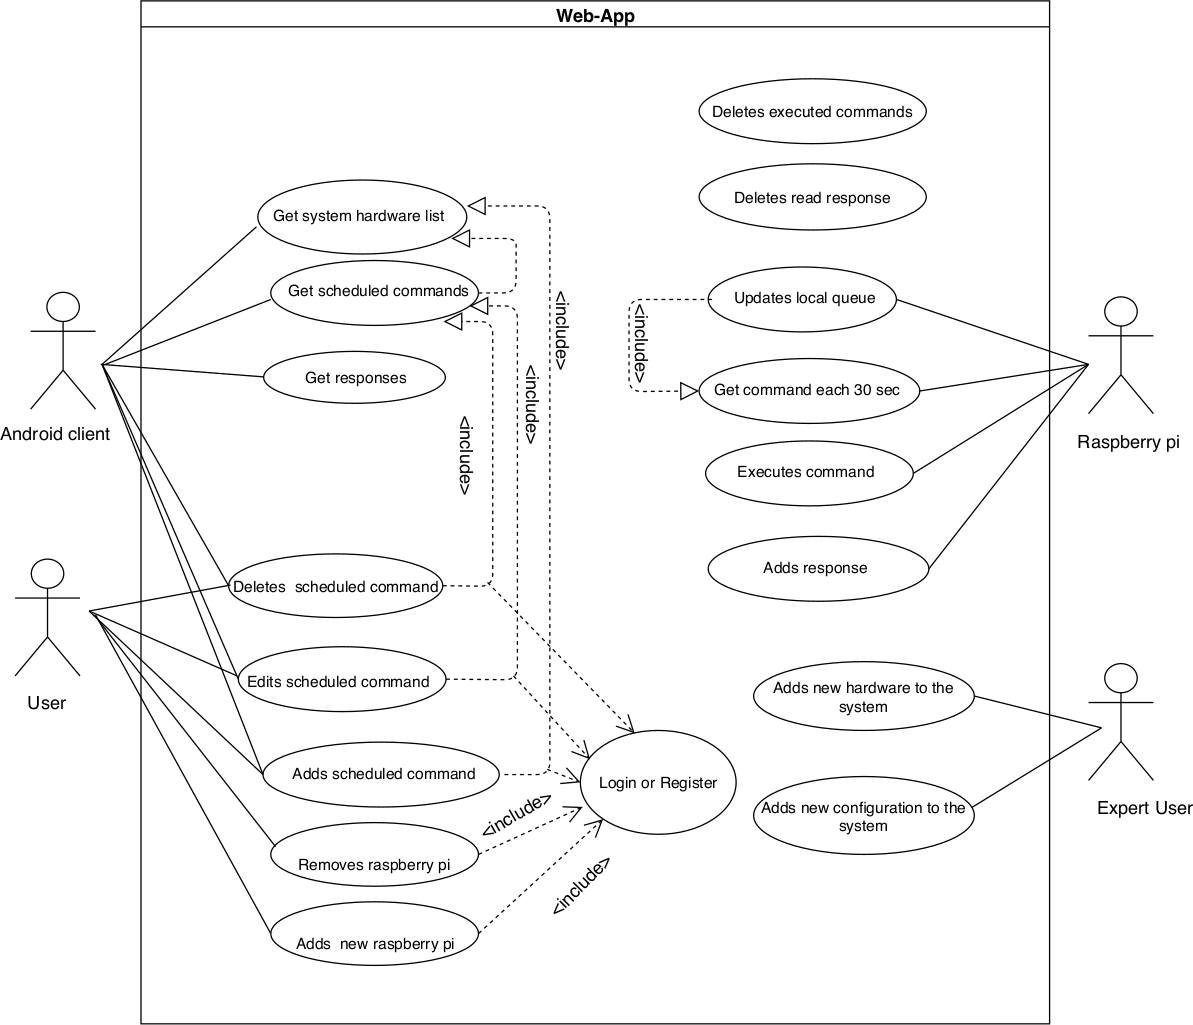
\includegraphics[width=\linewidth]{img/diagram_usecase.png}
			\caption{Use case diagram}
			\label{fig:diagram_usecase}
		\end{figure}
		\subsection{Flowchart Diagram}
		
		\begin{figure}[H]
			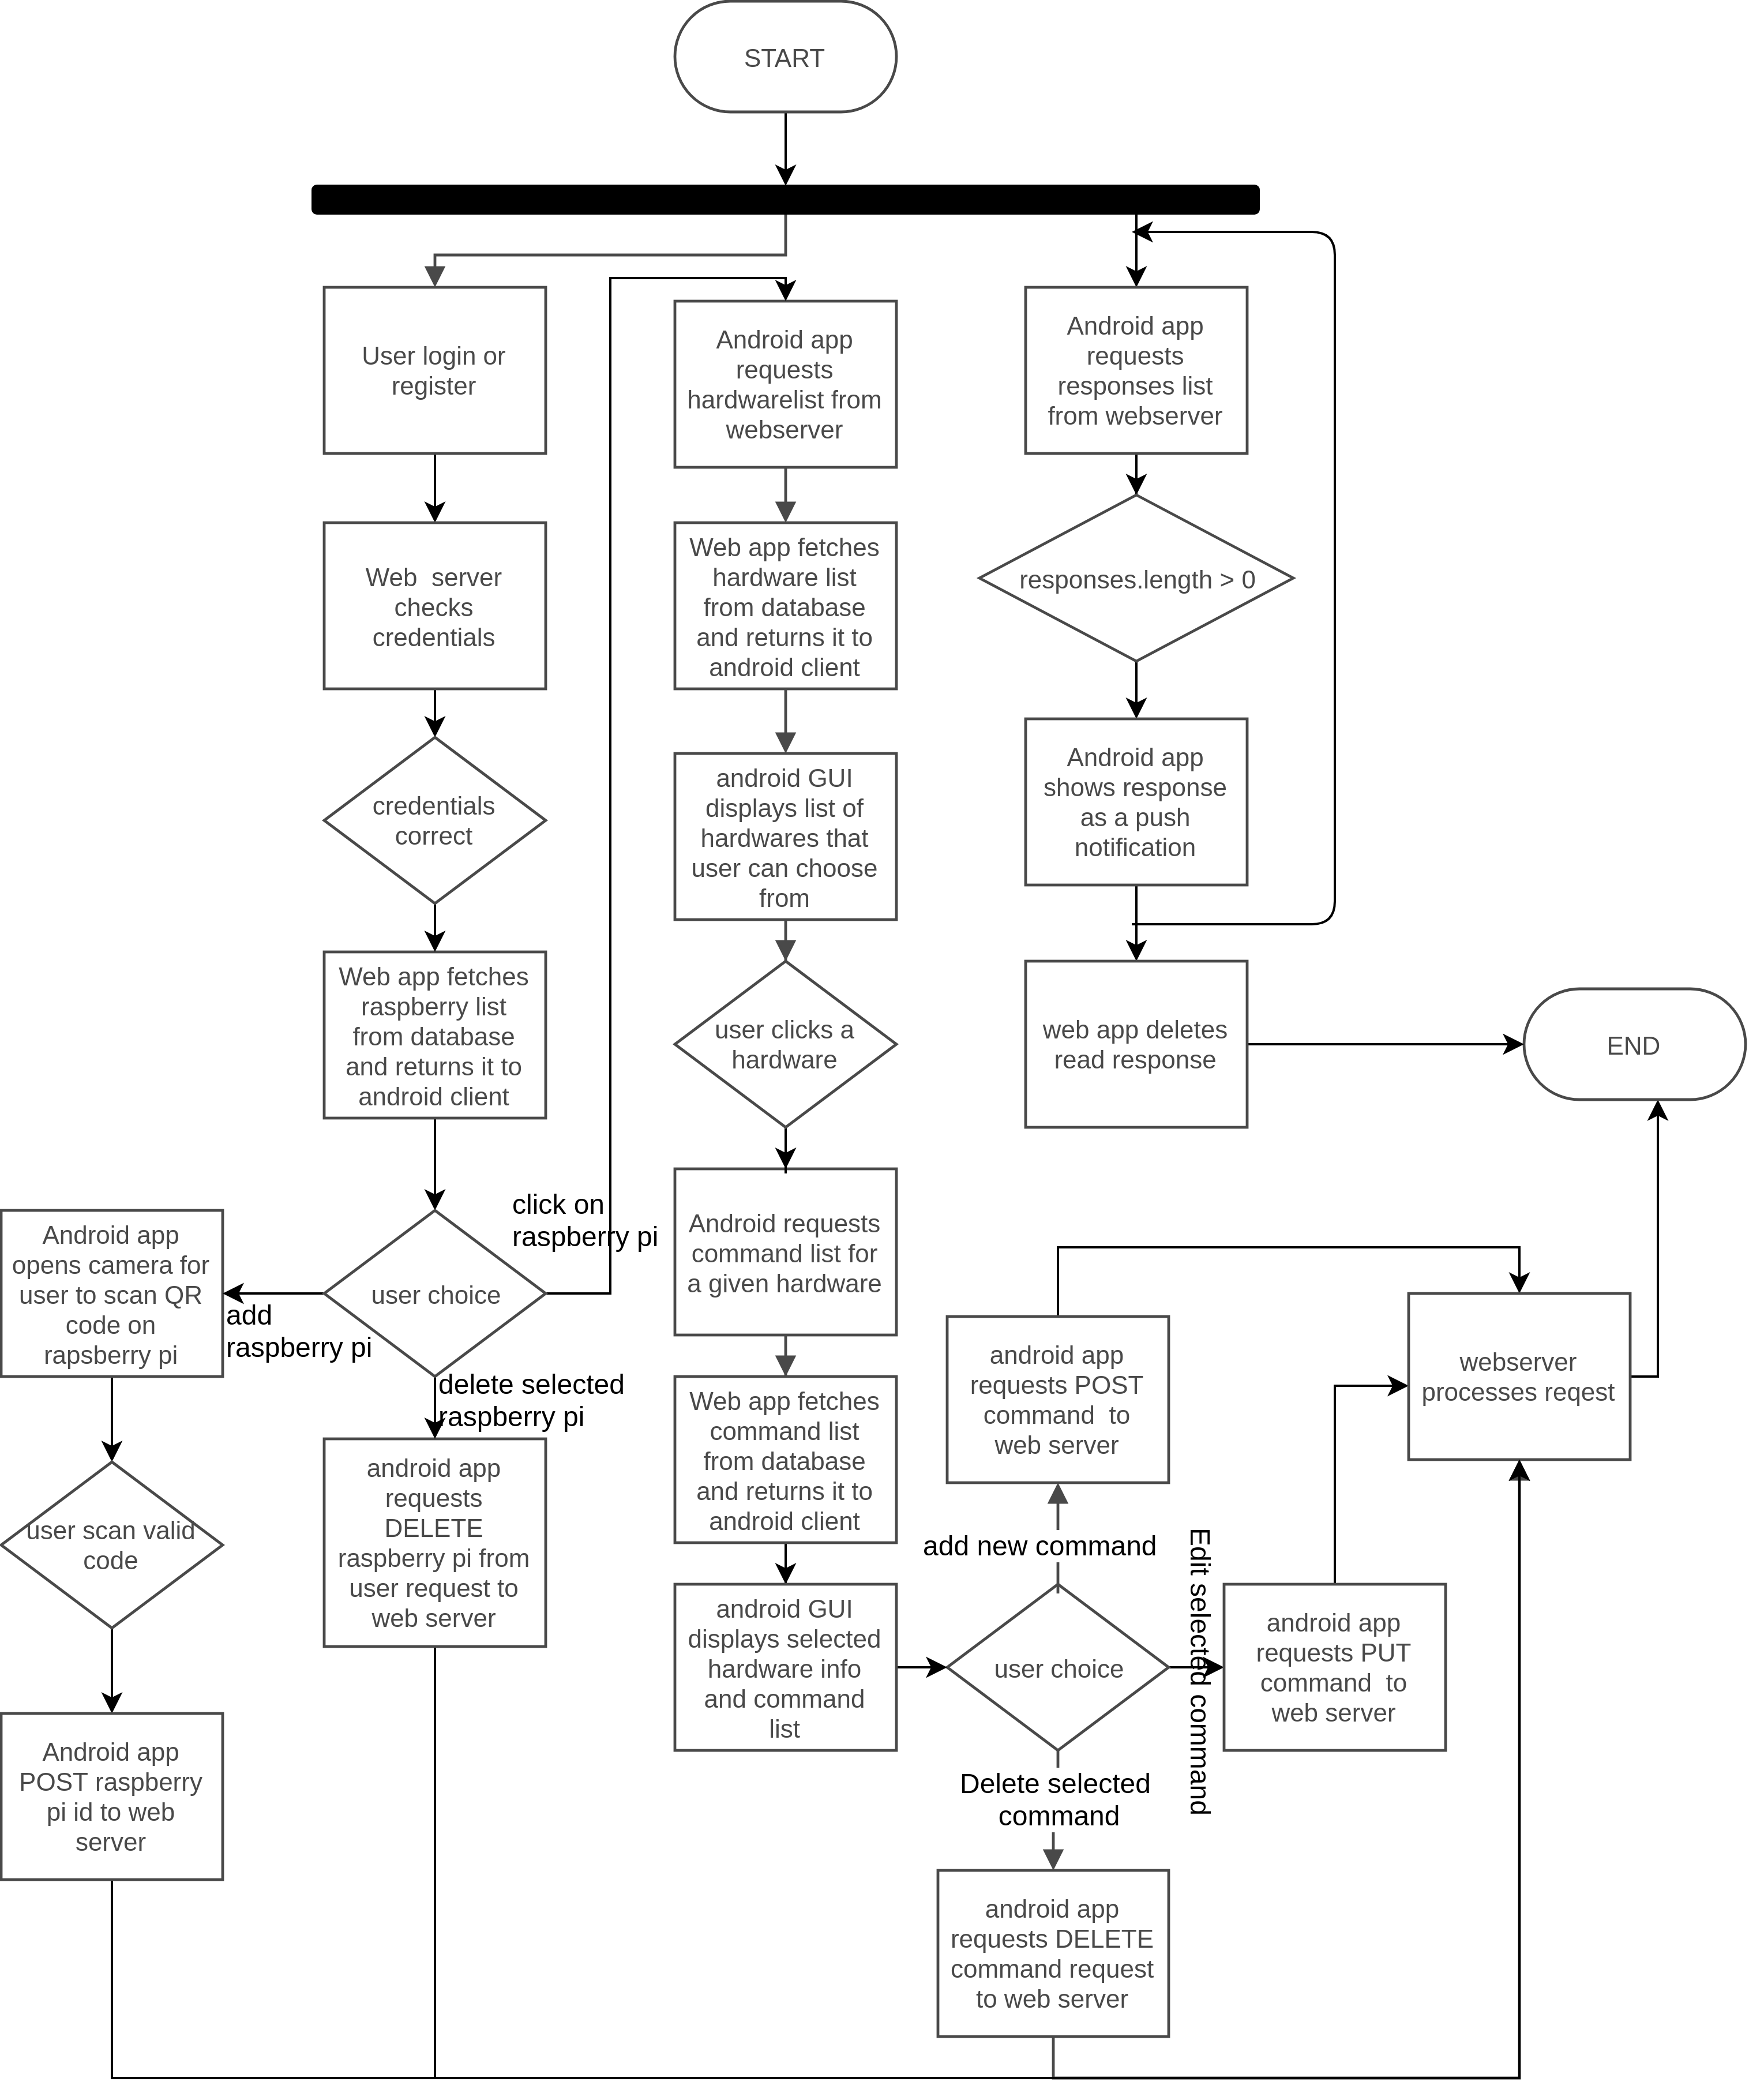
\includegraphics[width=\linewidth]{img/flowchart_android.png}
			\caption{Flow chart - Android app}
			\label{fig:ig:flow_android}
		\end{figure}
		\begin{figure}[H]
			\centering
			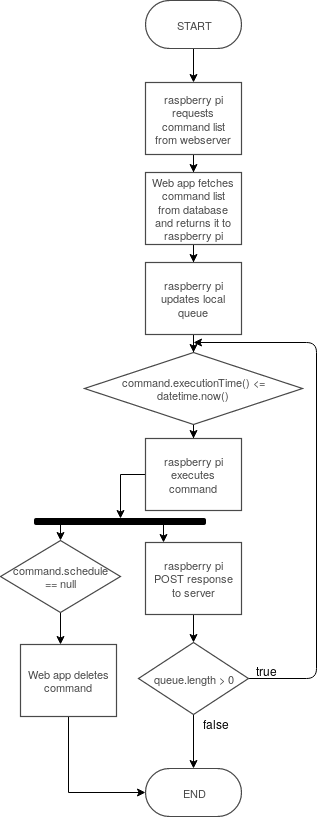
\includegraphics[width=.65\linewidth]{img/flowchart_raspberry.png}
			\caption{Flow chart - Raspberry pi}
			\label{fig:ig:flow_rasp}
		\end{figure}
\end{document}
	